\documentclass[11pt,a4paper]{article}
\usepackage[margin=1in]{geometry}
\usepackage[T1]{fontenc}
\usepackage{lmodern}
\usepackage{microtype}
\usepackage{booktabs,array,tabularx,longtable,multirow}
\usepackage{amsmath,amssymb}
\usepackage{graphicx}
\usepackage{xcolor}
\usepackage{tikz}
\usetikzlibrary{arrows.meta,positioning,decorations.pathreplacing,shapes.geometric,fit,calc}
\usepackage[most]{tcolorbox}
\usepackage{enumitem}
\usepackage{fancyhdr}
\usepackage{caption}
\usepackage{float}
\usepackage{tocloft}
\cftsetindents{section}{0em}{2.4em}
\cftsetindents{subsection}{2.4em}{3.2em}
\usepackage[hidelinks,bookmarks=true]{hyperref}

\graphicspath{{../docs/figures/}}

% ------------------------------------------------------------ look and feel
\definecolor{accent}{HTML}{1F4E79}
\definecolor{plainc}{HTML}{2E75B6}
\definecolor{keyc}{HTML}{2E7D32}
\definecolor{exc}{HTML}{B26A00}
\definecolor{warnc}{HTML}{B71C1C}
\definecolor{srcc}{HTML}{555555}

\setlength{\parindent}{0pt}
\setlength{\parskip}{5pt}
\setlist{itemsep=2pt,topsep=3pt,parsep=2pt}
\renewcommand{\arraystretch}{1.15}
\captionsetup{font=small,labelfont=bf}
\sloppy
\emergencystretch=2em

\pagestyle{fancy}
\fancyhf{}
\fancyhead[L]{\small\textcolor{srcc}{BitFlip: complete study guide}}
\fancyhead[R]{\small\textcolor{srcc}{\leftmark}}
\fancyfoot[C]{\small\thepage}
\renewcommand{\headrulewidth}{0.3pt}

\newtcolorbox{plain}{enhanced,breakable,colback=plainc!6,colframe=plainc,
  boxrule=0.6pt,arc=2pt,left=6pt,right=6pt,top=4pt,bottom=4pt,
  title=In plain words,fonttitle=\bfseries\small,coltitle=white,colbacktitle=plainc}
\newtcolorbox{keyidea}{enhanced,breakable,colback=keyc!6,colframe=keyc,
  boxrule=0.6pt,arc=2pt,left=6pt,right=6pt,top=4pt,bottom=4pt,
  title=Key idea,fonttitle=\bfseries\small,coltitle=white,colbacktitle=keyc}
\newenvironment{worked}[1][Worked example]{%
  \begin{tcolorbox}[enhanced,breakable,colback=exc!6,colframe=exc,
  boxrule=0.6pt,arc=2pt,left=6pt,right=6pt,top=4pt,bottom=4pt,
  title={#1},fonttitle=\bfseries\small,coltitle=white,colbacktitle=exc]}%
  {\end{tcolorbox}}
\newenvironment{careful}[1][Be careful here]{%
  \begin{tcolorbox}[enhanced,breakable,colback=warnc!5,colframe=warnc,
  boxrule=0.6pt,arc=2pt,left=6pt,right=6pt,top=4pt,bottom=4pt,
  title={#1},fonttitle=\bfseries\small,coltitle=white,colbacktitle=warnc]}%
  {\end{tcolorbox}}

% identifiers, file names, code: underscores and friends print literally
\DeclareRobustCommand{\code}[1]{\texttt{\detokenize{#1}}}
% where a fact came from
\newcommand{\src}[1]{\par\smallskip{\footnotesize\textcolor{srcc}{\textit{Source: #1}}}}
\newcommand{\term}[1]{\textbf{\textit{#1}}}

% numbers used all the time
\newcommand{\ee}[1]{\texttt{#1}}

\title{\textbf{BitFlip}\\[4pt]\Large A complete guide to the project\\ and to the TreeFI paper it builds on}
\author{Prepared for Peeyush Agarwal\\[2pt]\small CS496 Undergraduate Project, Indian Institute of Technology Kanpur}
\date{6 October 2026}

\begin{document}
\maketitle
\thispagestyle{empty}

\begin{abstract}
\noindent This guide explains your whole project, \emph{Reliability-Aware Fault Injection for
Microscaling-Based DNNs}, from the first idea to the last result, and it explains the TreeFI
paper (Bires, Traiola, Kritikakou and Fromont, ICCAD 2026) that your project builds on. It starts
from zero: what a neural network stores, what a bit flip is, what microscaling formats are. Then
it explains how the tool \code{mxfi} was built and how every experiment was run, tells the work
in the order it happened, with the numbers, and ends with the corrections you made, the design
guidance, the limits of the study, and practice questions for a viva.

\medskip\noindent Every number here comes from your repository (the report, \code{docs/findings.md},
the code, the result files) or from the TreeFI paper. Where a statement is my own explanation
or interpretation rather than something written in those sources, I say so.
\end{abstract}

\vspace{4pt}
\begin{plain}
\textbf{How to use this guide.} Part~I teaches the background. If you already know it, skip to
Part~II (the TreeFI paper) or Part~III (how your project works). Part~IV is the story with all the
results, and Part~V is the summary you would use to explain the project to someone else.
Part~VI has viva questions, a glossary, a cheat sheet of key numbers and a list of items to double-check.
Coloured boxes: \textcolor{plainc}{blue} = plain-language restatement, \textcolor{keyc}{green} = the
key idea, \textcolor{exc}{orange} = a worked example with real numbers, \textcolor{warnc}{red} = a trap or
caveat.
\end{plain}

\newpage
\tableofcontents
\newpage

\section*{The whole project on one page}
\addcontentsline{toc}{section}{The whole project on one page}
\markboth{The whole project on one page}{The whole project on one page}

\textbf{The question.} A neural network's weights and the values it computes while running
(activations) sit in memory. Sometimes a single bit in memory flips by accident. In an ordinary
number format, a flipped bit damages one number. In \emph{microscaling} (MX) formats, a block of
32 numbers shares one 8-bit scale, so a flip in that scale damages all 32 numbers at once. How much
do these flips actually hurt a network's predictions, and which formats, bits, layers and tensors
are most dangerous?

\textbf{What you built.} A fault-injection tool called \code{mxfi}. It encodes weights and activations
into real MX bit patterns, flips a chosen bit in an element or in a scale, decodes, runs the network,
and compares the predictions with the fault-free ones.

\textbf{What you ran.} About 60 trained networks (ResNet8, RepVGG-A0, a small Vision Transformer;
CIFAR-10 and CIFAR-100), five element formats, block sizes 8 to 64, weights and activations.
Roughly 1.44 million sampled weight faults in 119 campaigns, two \emph{exhaustive} campaigns that
flip every single stored bit of a ResNet8 (1.12 million injections), 390{,}000 multi-bit injections,
and further campaigns for activations, a NaN guard and CIFAR-100. The work ran on your laptop and on a
two-A100 server at IIT Kanpur.

\textbf{What you found.}
\begin{enumerate}
\item Formats with the same accuracy differ in fault vulnerability by up to three orders of magnitude.
 Measured per inference, e3m2 $<$ e4m3 $<$ e5m2 on every network tested.
\item The main cause is the NaN/Infinity codes of the 8-bit formats. On the larger networks 97 to 100\%
 of element damage comes from flips that land on such a code. Decoding those codes as zero on read cuts
 element damage by at least $29\times$ on RepVGG and the transformer.
\item A fault in the shared scale does $13\times$ to over $1000\times$ the damage of a fault in an element.
\item The usual ``did any test image change?'' metric mostly measures whether the test set contains a
 borderline image. You replaced it with a per-inference rate.
\item The severity score in your proposal does not predict failures. A gradient-based score does, and sampling
 with it needs $57$ to $120\times$ fewer injections.
\item Both open design choices in the proposal are settled: single-bit injection is enough, and exact
 enumeration of the code table beats TreeFI-style learned value intervals.
\end{enumerate}

\textbf{What you corrected along the way.} Eleven earlier conclusions were revised or withdrawn,
for reasons that come down to three causes: a misleading metric, too few trained networks, and
mismatched checkpoints and a codec bug. Section~\ref{sec:mistakes} lists all of them.

\textbf{What was not done.} ImageNet and DeiT were not reachable from any machine you could use, so
CIFAR-100 stands in for them. The optional small language model and MXINT8 were not studied.

\medskip
\begin{center}
\small
\begin{tabular}{@{}lr@{}}
\toprule
Report & 13 pages, \code{docs/report.pdf} \\
Findings log & 72 numbered findings, \code{docs/findings.md} \\
Library & \code{mxfi/}: 11 modules plus \code{__init__}, about 2{,}300 lines \\
Experiment scripts & \code{experiments/}: 29 scripts, about 5{,}200 lines \\
Tests & 4 files, about 1{,}100 lines \\
Repository & \code{github.com/peeyushagarwal2004/CS496_UGP} \\
\bottomrule
\end{tabular}
\end{center}
\src{README.md, docs/report.tex, docs/findings.md; line counts measured with wc on the repository.}

\newpage

\part{Foundations}

\section{Neural networks in five minutes}
\markboth{Neural networks}{Neural networks}

\subsection{What a network is, for this project}
An image classifier such as ResNet8 takes a picture and outputs a list of scores, one per class
(``airplane'', ``cat'', and so on). The class with the highest score is the prediction. Everything the
network knows is stored in numbers:
\begin{itemize}
\item \term{Weights} are fixed numbers learned during training. A small ResNet8 has about 78{,}000 of them,
 RepVGG-A0 about 7 million, your vision transformer about 2.7 million. They sit in memory the whole time
 the network is deployed.
\item \term{Activations} are temporary numbers. When one picture goes through the network, every layer
 computes new values from the previous layer's values. These are held in buffers just for that one picture.
\end{itemize}
A \term{layer} (a convolution or a fully connected layer) multiplies its input activations by its weights
and adds the results. Many layers stacked make the network.

\subsection{Training versus inference}
\term{Training} adjusts the weights so predictions become correct. \term{Inference} means using the finished
network to classify new pictures. Your whole project is about inference: you train a network once, then
study what happens when stored values are corrupted while it is being used.

\subsection{Words you will see all the time}
\begin{description}[leftmargin=2.2cm,style=nextline]
\item[Top-1 accuracy] The fraction of test pictures where the highest-scoring class is the correct one.
\item[Logits] The raw output scores, one per class, before any normalisation.
\item[Margin] The gap between the highest and the second-highest logit for one picture,
 $m = z_{(1)} - z_{(2)}$. A small margin means the network is nearly undecided between two classes.
 This quantity turns out to matter a great deal in your results.
\item[Prediction changed] A picture whose predicted class differs from what the fault-free network predicted
 (not from the true label). Your project measures how often a fault changes predictions.
\item[Seed] A number that fixes the random choices made during training (starting weights, order of
 pictures). Two networks with the same design and different seeds are two different trained networks that
 reach nearly the same accuracy but differ in many details. Seeds matter a lot later.
\item[CIFAR-10 / CIFAR-100] Small image datasets: $32\times32$ colour pictures. CIFAR-10 has 10 classes
 (60{,}000 images), CIFAR-100 has 100 classes with ten times fewer images per class, so it is a harder task.
\end{description}

\subsection{The three networks you used}
\begin{itemize}
\item \textbf{ResNet8}: the MLPerf Tiny image-classification network. A $3\times3$ convolution at the start
 (the ``stem''), three residual blocks, and a linear layer at the end: eight weight layers on the main path
 plus two $1\times1$ shortcut convolutions, ten quantised layers in all. At width 16 it has 78{,}042
 parameters. ``Width'' is the number of channels in the first layer; you trained widths 8, 16, 24, 32, 48
 (20 thousand to 692 thousand parameters).
\item \textbf{RepVGG-A0}: a plain stack of $3\times3$ convolutions. During training each block has three
 parallel branches ($3\times3$, $1\times1$, identity); for deployment the branches are fused into one
 $3\times3$ convolution. About 7.0 million parameters after fusion.
\item \textbf{A small Vision Transformer (ViT)}: the width and head count of DeiT-Tiny (192 dimensions,
 3 heads), depth 6, $4\times4$ patches, 2.7 million parameters. DeiT is the transformer family used in
 the TreeFI paper and named in your proposal; yours is a smaller version trained from scratch on CIFAR.
\end{itemize}

\section{Numbers inside a computer}
\markboth{Numbers in a computer}{Numbers in a computer}

\subsection{Bits}
A \term{bit} is a 0 or a 1. A number is stored as a row of bits. $n$ bits can name $2^n$ different things:
8 bits give 256 codes, 6 bits give 64, 4 bits give 16.

\subsection{FP32, the normal format}
Ordinary computation uses \term{FP32} (32-bit floating point), laid out as
\[
\underbrace{1}_{\text{sign}}\;|\;\underbrace{8}_{\text{exponent}}\;|\;\underbrace{23}_{\text{mantissa}}.
\]
The value is $(-1)^{\text{sign}}\times(1+\text{mantissa}/2^{23})\times2^{\text{exponent}-127}$. It is scientific
notation in base 2: the exponent says how big the number is, the mantissa says exactly where inside that size.
Every FP32 number is \emph{self-contained}: all its information lives in its own 32 bits. So if one bit of a
FP32 weight flips, exactly that one weight changes.

\subsection{Why shrink the numbers: quantisation}
32 bits per weight is a lot of memory, and moving memory costs energy and time. \term{Quantisation} stores
each number in fewer bits (8, 6 or 4) at the price of rounding error. A quantised network is slightly
different from the original, but if it is done well, accuracy barely changes.

\subsection{Fake quantisation, which is what your tool does}
Your tool runs everything in FP32 on a normal PC, but \emph{before} using a weight it rounds it to the value
the MX format could actually store. This is called \term{fake quantisation}: the network computes with exactly
the numbers an MX accelerator would use, though the arithmetic is done in FP32. Faults are injected in the
stored bit pattern, then decoded to FP32 and used.

\section{Microscaling (MX) formats}
\markboth{Microscaling}{Microscaling}

\subsection{The idea}
MX is defined by the OCP Microscaling Formats specification (and the paper by Rouhani et al., 2023). Group the
numbers of a tensor into \term{blocks} of $K$ consecutive numbers (usually $K=32$). For each block store
\begin{itemize}
\item one \term{shared scale} $X$: 8 bits, shared by all $K$ numbers; and
\item one small \term{element code} per number: 4, 6 or 8 bits.
\end{itemize}
The real value of element $i$ is
\begin{equation}\label{eq:mx}
v_i \;=\; \operatorname{decode}(\text{code}_i)\;\times\;2^{\,X-127}.
\end{equation}

\begin{plain}
Think of a price list of 32 items with one note at the top: ``all prices in thousands''. Each row only
stores a short number, and the single note says how to read all of them. That saves a lot of memory. The
danger is obvious: if the note gets corrupted, \emph{all 32 prices} become wrong at once.
\end{plain}

\subsection{The scale is E8M0}
The scale byte is in a format called \term{E8M0}: 8 exponent bits and no mantissa bits. So the scale is always
an exact power of two: byte $X$ means $2^{X-127}$. Byte 127 means $\times1$, byte 128 means $\times2$, byte 118
means $2^{-9}$. Bytes 0 to 254 are normal scales (so the range is $2^{-127}$ to $2^{127}$). \textbf{Byte 255 is
reserved to mean NaN} (not a number, an error value).

\subsection{Memory saved}
A block of 32 numbers with 8-bit codes needs $8+32\times8=264$ bits, which is $8.25$ bits per number instead
of 32. That is the benefit.

\subsection{Two fault sites and the blast radius}
This is the central structural fact of your project (it comes straight from your proposal).
\begin{center}
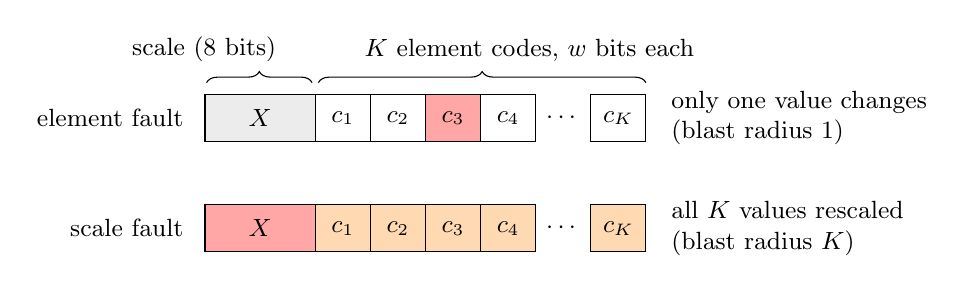
\begin{tikzpicture}[font=\small,
  cell/.style={draw, minimum width=7mm, minimum height=6mm, inner sep=0pt},
  scl/.style={draw, minimum width=14mm, minimum height=6mm, inner sep=0pt}]
  \node[anchor=east] at (-0.15,0) {element fault};
  \node[scl, fill=gray!15] at (0.7,0) {$X$};
  \node[cell] at (1.75,0) {$c_1$};
  \node[cell] at (2.45,0) {$c_2$};
  \node[cell, fill=red!35] at (3.15,0) {$c_3$};
  \node[cell] at (3.85,0) {$c_4$};
  \node at (4.55,0) {$\cdots$};
  \node[cell] at (5.25,0) {$c_K$};
  \node[anchor=west, align=left] at (5.8,0) {only one value changes\\(blast radius 1)};
  \node[anchor=east] at (-0.15,-1.4) {scale fault};
  \node[scl, fill=red!35] at (0.7,-1.4) {$X$};
  \foreach \x/\l in {1.75/c_1,2.45/c_2,3.15/c_3,3.85/c_4,5.25/c_K}
     \node[cell, fill=orange!30] at (\x,-1.4) {$\l$};
  \node at (4.55,-1.4) {$\cdots$};
  \node[anchor=west, align=left] at (5.8,-1.4) {all $K$ values rescaled\\(blast radius $K$)};
  \draw[decorate, decoration={brace, amplitude=4pt}] (0.02,0.45) -- (1.36,0.45)
    node[midway, above=4pt, xshift=-7mm] {scale (8 bits)};
  \draw[decorate, decoration={brace, amplitude=4pt}] (1.44,0.45) -- (5.6,0.45)
    node[midway, above=4pt, xshift=6mm] {$K$ element codes, $w$ bits each};
\end{tikzpicture}
\captionof{figure}{One MX block and its two fault sites. Red is the flipped word; orange are the values it changes.}
\end{center}

A flip of bit $j$ of the scale multiplies every value in the block by $2^{\pm2^{j}}$: bit 0 means $\times2$ or
$\div2$, bit 1 means $\times4$, bit 2 means $\times16$, bit 3 means $\times256$, \ldots, bit 7 means $\times2^{128}$.
That is why the scale is so dangerous.

\src{proposal PDF Sec.~1 and 3; mxfi/formats.py (E8M0 definition); report Sec.~2.}

\section{The five element formats}
\markboth{Element formats}{Element formats}

\subsection{Anatomy of an element code}
An element code has three groups of bits. Names such as \ee{e4m3} mean: \textbf{e}xponent \textbf{4} bits,
\textbf{m}antissa \textbf{3} bits, plus one sign bit, 8 bits in all. The names MXFP8, MXFP6 and MXFP4
count the total bits per element.

\begin{center}
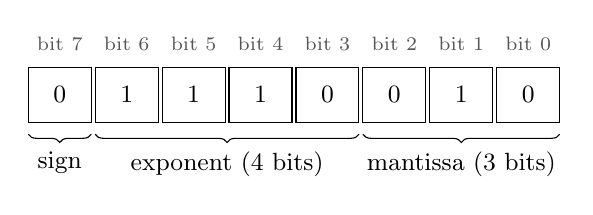
\begin{tikzpicture}[font=\small, bit/.style={draw, minimum width=8mm, minimum height=7mm, inner sep=0pt}]
  \foreach \i/\v in {0/0,1/1,2/1,3/1,4/0,5/0,6/1,7/0}{
    \node[bit] at (\i*0.85,0) {\v};
  }
  \foreach \i/\b in {0/7,1/6,2/5,3/4,4/3,5/2,6/1,7/0}{
    \node[font=\scriptsize, text=srcc] at (\i*0.85,0.65) {bit \b};
  }
  \draw[decorate,decoration={brace,mirror,amplitude=3pt}] (-0.4,-0.5) -- (0.4,-0.5) node[midway,below=3pt] {sign};
  \draw[decorate,decoration={brace,mirror,amplitude=3pt}] (0.45,-0.5) -- (3.8,-0.5) node[midway,below=3pt] {exponent (4 bits)};
  \draw[decorate,decoration={brace,mirror,amplitude=3pt}] (3.85,-0.5) -- (6.35,-0.5) node[midway,below=3pt] {mantissa (3 bits)};
\end{tikzpicture}
\captionof{figure}{The bits of an \ee{e4m3} code; the example shown is \ee{01110010}.}
\end{center}

\subsection{Decoding a code by hand}
For a code with exponent field $e$ and mantissa field $f$ (an $M$-bit number), when $e\neq0$:
\begin{equation}\label{eq:decode}
\operatorname{decode}=(-1)^{s}\,\Bigl(1+\frac{f}{2^{M}}\Bigr)\,2^{\,e-\mathrm{bias}},\qquad
\mathrm{bias}=2^{\text{exp\_bits}-1}-1 .
\end{equation}
When $e=0$ the number is \term{subnormal}: there is no leading ``1+'', which is how the format gets zero and very
tiny numbers.

\begin{worked}[Worked example: decode the e4m3 code 01110010]
Sign bit $=0$ (positive). Exponent bits \ee{1110} $=14$. Mantissa bits \ee{010} $=2$, with $M=3$. The bias of
e4m3 is $2^{3}-1=7$. So
\[
\Bigl(1+\tfrac{2}{8}\Bigr)\times2^{14-7}=1.25\times128=\mathbf{160}.
\]
The table inside \code{mxfi/formats.py} also gives 160.0 (checked by running it).
\end{worked}

\subsection{What bias is}
The exponent field only stores $0,1,2,\dots$, but we need small numbers like $2^{-3}$ too. So the stored value means
``exponent plus bias'', and the bias (7 for e4m3, 15 for e5m2, 3 for e3m2, 1 for e2m3 and e2m1) is subtracted
back out.

\subsection{The smallest format on one card: e2m1}
The 4-bit format has only 16 codes. All of them (computed from your \code{formats.py}):
\begin{center}
\small
\begin{tabular}{cc@{\hspace{2cm}}cc}
\toprule
code & value & code & value \\
\midrule
0000 & 0 & 1000 & $-0$ \\
0001 & 0.5 & 1001 & $-0.5$ \\
0010 & 1 & 1010 & $-1$ \\
0011 & 1.5 & 1011 & $-1.5$ \\
0100 & 2 & 1100 & $-2$ \\
0101 & 3 & 1101 & $-3$ \\
0110 & 4 & 1110 & $-4$ \\
0111 & \textbf{6} & 1111 & $-6$ \\
\bottomrule
\end{tabular}
\end{center}
With 4 bits you can only say $0, 0.5, 1, 1.5, 2, 3, 4, 6$ and their negatives. That is why the largest value is 6.
The shared scale then slides this tiny menu up or down to wherever the real weights are.

\subsection{The five formats side by side}
\begin{center}
\small
\begin{tabular}{lllcccc}
\toprule
format & family & sign/exp/man & bias & largest value & codes & special codes \\
\midrule
e4m3 & MXFP8 & 1/4/3 & 7  & 448    & 256 & 2 (NaN) \\
e5m2 & MXFP8 & 1/5/2 & 15 & 57{,}344 & 256 & 8 (2 Inf, 6 NaN) \\
e3m2 & MXFP6 & 1/3/2 & 3  & 28     & 64  & none \\
e2m3 & MXFP6 & 1/2/3 & 1  & 7.5    & 64  & none \\
e2m1 & MXFP4 & 1/2/1 & 1  & 6      & 16  & none \\
\bottomrule
\end{tabular}
\end{center}
How the largest values come out: for e4m3 the biggest exponent field is 15 and the biggest allowed mantissa is
\ee{110}, so $1.75\times2^{15-7}=448$ (mantissa \ee{111} at exponent 15 is reserved for NaN). For e3m2:
$1.75\times2^{7-3}=28$. For e5m2 the exponent field 31 is reserved, so the biggest normal exponent is 30:
$1.75\times2^{30-15}=57{,}344$.

\textbf{Range versus precision.} More exponent bits means a wider range; more mantissa bits means finer steps.
e5m2 reaches 57{,}344 but can only name 4 values between consecutive powers of two; e2m3 reaches only 7.5 but
can name 8 values between powers of two. A code alone only covers a narrow window; the shared scale slides
the window to where the real weights are.

\subsection{Special codes: the single most important column}
Standard floating point reserves some patterns to mean ``not a number'' (NaN) or infinity. Your code printed
the exact patterns:
\begin{itemize}
\item \textbf{e4m3}: \ee{01111111} and \ee{11111111} (exponent \ee{1111} and mantissa \ee{111}, positive and negative):
 2 NaN codes.
\item \textbf{e5m2}: exponent \ee{11111} is special. Mantissa \ee{00} means $\pm\infty$ (2 codes); mantissa
 \ee{01}, \ee{10}, \ee{11} means NaN (6 codes). Total 8.
\item \textbf{e3m2, e2m3, e2m1}: none. With only 64 or 16 codes, every pattern was kept as a real number.
\end{itemize}

\begin{worked}[Worked example: one flip lands on NaN (computed with your code)]
Take the e4m3 code \ee{01111011}. Its value at unit scale is 352. Flipping each of its 8 bits in turn gives:

\smallskip
\begin{center}\small
\begin{tabular}{ccc}
\toprule
bit flipped & new code & new value \\
\midrule
0 & 01111010 & 320 \\
1 & 01111001 & 288 \\
\textbf{2} & \textbf{01111111} & \textbf{NaN} \\
3 & 01110011 & 176 \\
4 & 01101011 & 88 \\
5 & 01011011 & 22 \\
6 & 00111011 & 1.375 \\
7 & 11111011 & $-352$ \\
\bottomrule
\end{tabular}
\end{center}
Seven of the eight flips just give another ordinary number (some very different, but finite). Bit 2
lands exactly on the NaN pattern. In e5m2 the same code is its largest number (57{,}344) and the same flip also
gives NaN. Note that bit 7, the sign, gives $-352$: a sign flip can \emph{never} reach NaN, because the NaN
pattern needs the magnitude bits all equal to 1 and a sign flip does not touch them.
\end{worked}

\subsection{Why NaN is so much worse than a large wrong number}
\begin{itemize}
\item A wrong but finite number changes the output a little, and a large network often absorbs that.
\item NaN contaminates everything it touches ($\mathrm{NaN}+x=\mathrm{NaN}$ and $\mathrm{NaN}\times x=\mathrm{NaN}$).
 One NaN weight makes the layer's output NaN, which feeds the next layer, and so on until all the final scores
 are NaN and the ``prediction'' means nothing.
\item For a \emph{weight} fault the bad weight stays in memory, so every image is ruined. For an
 \emph{activation} fault only that one image is affected.
\end{itemize}
Formats without special codes (e3m2, e2m3, e2m1) cannot suffer this at element level: every flip yields some finite number.

\src{report Sec.~2.1 (the formats table), mxfi/formats.py, and a run of mxfi on 6 October 2026.}

\section{Choosing the scale: the OCP rule and the fit rule}
\markboth{Choosing the scale}{Choosing the scale}

\subsection{The problem}
Real weights may be 0.0007 or 480, but codes only name a small menu (up to 448 for e4m3, up to 6 for e2m1). The
scale slides the menu. Given a block of numbers, which scale byte should be stored? A rule is needed.

\subsection{The OCP rule}
Line the biggest number in the block up with the top of the format's range:
\begin{equation}\label{eq:ocp}
X \;=\; \operatorname{clamp}\bigl(\lfloor\log_2\max_i|v_i|\rfloor-e_{\max}\bigr)+127\quad(\text{as stored byte}),
\end{equation}
where $e_{\max}=\lfloor\log_2(\text{largest value of the format})\rfloor$: e4m3 8, e5m2 15, e3m2 4, e2m3 2, e2m1 2
(computed).

\begin{worked}[Worked example (computed): the scale of one block]
Block of 8 numbers, e4m3, largest $|v|=0.71$. $\log_2 0.71=-0.49$ and its floor is $-1$. The exponent to use is
$-1-8=-9$; the stored byte is $-9+127=118$. Check: $0.71/2^{-9}=363.5$, which is inside the e4m3 menu (up to 448).
Elements are then rounded to the nearest representable code (ties to even): 363.5 becomes 352, i.e. $352\times2^{-9}=0.6875$.
\end{worked}

\subsection{What a binade is, and the clipping problem}
A \term{binade} is the range between two consecutive powers of two (for example 256 to 512). After the OCP rule
the block maximum always lands in $[2^{e_{\max}},2^{e_{\max}+1})$, the top binade. For e4m3 that is $[256,512)$, but the
biggest number the format can store is 448. A block maximum between 448 and 512 cannot be stored; it is
\term{clipped} (squashed) to 448.

\begin{worked}[Worked example (computed): clipping, OCP versus fit]
A block whose biggest value is 480, in e4m3.
\begin{center}\small
\begin{tabular}{lcl}
\toprule
rule & scale & what is stored \\
\midrule
OCP & $2^{0}$ & \textbf{448}, 96, 20, 1 \quad (480 was clipped) \\
fit & $2^{1}$ & \textbf{480}, 96, 20, 1 \quad (exact) \\
\bottomrule
\end{tabular}
\end{center}
With the block maximum at 511 (the worst case) OCP stores 448, an error of 12.33\%; fit stores 512, an error of 0.2\%.
\end{worked}

The worst-case clipping equals $1-\text{largest value}/\text{top of binade}$:
\begin{center}\small
\begin{tabular}{lccc}
\toprule
format & top binade & largest value & worst-case clip \\
\midrule
e4m3 & $[256,512)$ & 448 & 12.5\% \\
e5m2 & $[32768,65536)$ & 57344 & 12.5\% \\
e3m2 & $[16,32)$ & 28 & 12.5\% \\
e2m3 & $[4,8)$ & 7.5 & 6.25\% \\
e2m1 & $[4,8)$ & 6 & 25\% \\
\bottomrule
\end{tabular}
\end{center}
Only the block's largest values are affected; everything else is rounded normally.

\subsection{Why the spec does this, and your control rule ``fit''}
My reading (not a quote from the spec): lining the maximum up with the top of the range uses the format's full
range, so every weight gets the finest steps available, at the cost of possibly clipping the largest few values.
Your control rule \term{fit} picks the \emph{smallest scale at which nothing can clip}:
$X=\lceil\log_2(\max|v|/\text{largest value})\rceil$. It is the same as OCP or one step larger, and shifts the block
slightly down the menu, so the smallest weights are a little more likely to round to zero.

You implemented fit to check that format differences are not just clipping differences. Your first results show
why it mattered: at $K=32$, under OCP the 6-bit e2m3 got 0.8572 accuracy and the 8-bit e4m3 0.8508, so the smaller
format ``won''; under fit it was 0.8578 against 0.8610 and the order flipped back. e2m3 only looked better because
it clips less (6.25\% against 12.5\%).

\section{Faults}
\markboth{Faults}{Faults}

\subsection{Soft errors and the single-bit flip}
A \term{soft error} is a bit that changes without the hardware being broken. Typical causes are radiation
(a particle hitting a memory cell) or electrical noise. (The TreeFI paper states it the same way: ``soft errors
induced by radiation or electrical noise, may cause bit flips that silently corrupt intermediate computations
and alter the final prediction''.) The chip is fine afterwards; only the stored value was wrong.

The standard fault model, which your proposal adopts, is the \term{single-bit flip}: exactly one stored bit
changes. A stored bit may belong to a weight, to an activation, or to a shared scale.

\subsection{Possible outcomes of a flip}
\begin{enumerate}
\item \textbf{Masked}: nothing observable changes.
\item \textbf{Crash or detected error}: the program stops or reports a problem.
\item \textbf{SDC (silent data corruption)}: the program runs normally and gives a \emph{different answer}, with no warning.
\end{enumerate}
Your project is about the third case: does a prediction silently change?

\subsection{Persistent versus transient}
A fault in a \emph{weight} stays until the memory is rewritten, so it affects \emph{every} image processed in the
meantime. A fault in an \emph{activation} lives in a temporary buffer and affects only the image being processed.
This difference matters when comparing the two, and is the reason you needed a per-inference rate
(Section~\ref{sec:metrics}).

\subsection{A worked example of the two sites (computed)}
Eight numbers stored as one e4m3 block ($K=8$):
\begin{center}\small
\begin{tabular}{ll}
\toprule
original & 0.30, $-0.12$, 0.05, 0.71, $-0.44$, 0.02, 0.18, $-0.60$ \\
scale byte & 118, meaning $2^{-9}=0.00195$ \\
codes & \ee{01110010 11100111 01011101 01111011 11110110 01010010 01101100 11111010} \\
decoded & 0.3125, $-0.1172$, 0.0508, 0.6875, $-0.4375$, 0.0195, 0.1875, $-0.625$ \\
\bottomrule
\end{tabular}
\end{center}
The decoded numbers differ slightly from the originals because of rounding. Now flip one bit:
\begin{center}\small
\begin{tabular}{lp{8cm}}
\toprule
what is flipped & result \\
\midrule
fourth element (0.71), bit 6 (a top exponent bit) & only that number changes: $0.6875\to0.0027$; the other 7 are untouched \\
scale bit 0 & \textbf{all 8 numbers double}: $0.3125\to0.625$, $-0.117\to-0.234$, \ldots \\
scale bit 3 & \textbf{all 8 multiplied by 256}: $0.3125\to80$, $0.6875\to176$, $-0.625\to-160$ \\
scale bit 7 & \textbf{all 8 become about $10^{38}$}, the edge of the float32 range (larger values would overflow to infinity) \\
\bottomrule
\end{tabular}
\end{center}
A single flipped bit in a one-byte scale turned a block of small numbers into huge ones.

\subsection{A counting argument: why the scale matters even before measuring}
In one block there are 8 scale bits and $Kw$ element bits (with $w$ bits per element). If every stored bit is equally
likely to flip:
\begin{itemize}
\item scale flips: 8 bits $\times$ $K$ corrupted values each $=8K$;
\item element flips: $Kw$ bits $\times$ 1 corrupted value each $=Kw$.
\end{itemize}
The ratio is $8K:Kw=8:w$; $K$ cancels. With 8-bit elements it is $8:8$, so scales supply \emph{half} of all
corrupted values although they are only 3\% of the storage; with 4-bit elements it is $8:4$, two thirds.

\begin{center}\small
\begin{tabular}{lccc}
\toprule
 & $w=8$ & $w=6$ & $w=4$ \\
\midrule
share of storage that is scale, $K=8$ & 11.1\% & 14.3\% & 20.0\% \\
$K=16$ & 5.9\% & 7.7\% & 11.1\% \\
$K=32$ & 3.0\% & 4.0\% & 5.9\% \\
$K=64$ & 1.5\% & 2.0\% & 3.0\% \\
\bottomrule
\end{tabular}
\end{center}

\begin{careful}[A fair caveat]
This argument only counts \emph{how many values are touched}, not \emph{how badly}. Your measurements later
showed a scale flip does $13\times$ to over $1000\times$ more damage than an element flip, far more than the
$8:w$ count alone gives, because a scale flip also multiplies by a huge factor while many element flips barely change a
number. So the counting argument is a reason to suspect the scale matters, and the experiments supplied the size of the effect.
\end{careful}

\section{Fault injection and how failure is measured}
\label{sec:metrics}
\markboth{Fault injection}{Fault injection}

\subsection{Fault injection, golden runs and campaigns}
\term{Fault injection} (FI) means deliberately corrupting a stored value and observing what happens. The procedure:
\begin{enumerate}
\item Run the fault-free network on a fixed set of test images and record its predictions: the \term{golden} predictions.
\item Pick a fault: a layer, a site (element or scale), a position, a bit. Flip it.
\item Run the same images again and compare with the golden predictions.
\item Record what changed, then undo the flip.
\end{enumerate}
Repeating this for many faults is a \term{campaign}. The set of all possible faults is the \term{fault space}; for ResNet8
in e4m3 it has 638{,}624 single-bit faults.

\subsection{Exhaustive versus statistical}
\begin{itemize}
\item \textbf{Exhaustive FI} injects every fault. It gives the exact failure rate with no sampling error, but it is only affordable on small
 models. You did it twice, on ResNet8 (638{,}624 and 483{,}904 faults).
\item \textbf{Statistical FI (SFI)} injects a random sample and uses probability theory to say how close the sample's rate is to
 the true rate. Most of your campaigns use 3{,}000 uniformly sampled faults.
\end{itemize}
Both are used together in your project: the exhaustive runs validate the sampling.

\subsection{The two metrics}
Let $N=200$ be the number of evaluation images, $\hat y_i$ the golden prediction for image $i$ and $\hat y_i^{\varphi}$ the prediction
under fault $\varphi$.
\begin{itemize}
\item \textbf{Any-image SDC} (the conventional metric, and the one you used for the first three weeks):
\[
\mathrm{sdc}(\varphi)=\mathbf 1\Bigl[\textstyle\sum_{i}\mathbf 1[\hat y^{\varphi}_i\neq\hat y_i]>0\Bigr],
\]
the fault counts as failing if \emph{at least one} of the 200 predictions changed. The reported rate is the share of
faults that fail.
\item \textbf{Per-inference rate} (what you adopted):
\[
r(\varphi)=\frac1N\sum_i\mathbf 1[\hat y^{\varphi}_i\neq\hat y_i],\qquad
\text{rate}=\text{mean of }r(\varphi)\text{ over faults.}
\]
It answers: given one fault, what is the probability that a particular inference is wrong?
\item \textbf{Non-finite rate}: the share of faults whose output contained NaN or infinity.
\end{itemize}
Why the first metric turned out to be misleading is explained in Section~\ref{sec:phase-metric}. In short: it saturates
towards 1 as $N$ grows and mostly measures whether the 200 images contain a near-tie.

\subsection{Confidence intervals, in plain words}
Because a campaign samples faults, its rate is an estimate. A \term{95\% confidence interval} is a range that, in repeated experiments,
would contain the true value 95\% of the time. For a failure \emph{proportion} you used the \term{Wilson interval}: with $k$ failures in
$n$ trials, $\hat p=k/n$ and $z=1.96$,
\[
\frac{\hat p+\frac{z^2}{2n}\;\pm\;z\sqrt{\frac{\hat p(1-\hat p)}{n}+\frac{z^2}{4n^2}}}{1+\frac{z^2}{n}} .
\]
It stays inside $[0,1]$ and remains informative when $k=0$, unlike the textbook normal approximation. For the per-inference rate (a mean
of numbers between 0 and 1) you used a normal or bootstrap interval. These intervals only cover the uncertainty from \emph{which
faults} were sampled; they say nothing about which trained network or which images were used. That limitation matters a lot later.

\subsection{Stratified sampling and Neyman allocation}
If the failure rate differs a lot between groups (``strata'') of faults, sampling the groups equally wastes effort on the boring ones.
\term{Stratified sampling} splits the fault space into strata, samples each, and combines the results with weights $W_h$ equal to each stratum's share of the space:
\[
\hat p=\sum_h W_h\hat p_h,\qquad \operatorname{Var}(\hat p)=\sum_h W_h^{2}\frac{\sigma_h^{2}}{n_h},
\]
where $\sigma_h^2=p_h(1-p_h)$ for a yes/no outcome. Choosing $n_h$ to minimise the variance for a fixed total $n$ gives
\term{Neyman allocation}: $n_h\propto W_h\sigma_h$, so strata that are big and uncertain get more samples, and strata that are almost
certainly 0 or 1 get few. The \term{variance reduction} is the ratio $\operatorname{Var}_{\text{uniform}}/\operatorname{Var}_{\text{stratified}}$ at the same budget; a value of 10
means uniform sampling would need ten times the injections for the same precision. Your \code{mxfi/stats.py} and \code{mxfi/sampling.py}
implement this.

\subsection{Margins and ``near-ties'' (preview)}
Recall that the margin $m$ is the gap between the top two logits. An image with a tiny margin is a \term{near-tie}: almost any perturbation flips its
prediction. If the evaluation set happens to contain a near-tie in one particular quantised network, the any-image metric records
a failure for almost every fault, whether or not the fault is really dangerous. This single idea explains several of the reversals in
your results.

\part{The TreeFI paper}

This part explains the paper in the file \code{hal.pdf} that you attached. It is the prior work your project cites. Everything in
this part is taken from that paper; where I add my own explanation or comparison with your project I mark it.

\section{The paper at a glance}
\markboth{TreeFI at a glance}{TreeFI at a glance}

\begin{center}
\small
\begin{tabular}{@{}lp{11cm}@{}}
\toprule
Title & \emph{TreeFI: Value-Aware Statistical Fault Injection for Deep Neural Networks} \\
Authors & Noam Bires, Marcello Traiola, Angeliki Kritikakou, Elisa Fromont (Inria, IRISA, Univ Rennes, CNRS, Rennes, France) \\
Venue & ICCAD 2026 (IEEE/ACM International Conference on Computer-Aided Design), November 2026, San Jose, USA \\
Archive & HAL id \code{hal-05704925}, submitted 27 July 2026, licence CC BY 4.0 \\
Code & \code{gitlab.inria.fr/nbires/treefi} \\
Length & 10 pages including the HAL cover page \\
\bottomrule
\end{tabular}
\end{center}

\begin{keyidea}
\textbf{One sentence.} When you test a neural network by flipping random bits, \emph{what a flip does depends strongly on the value
that is being corrupted}; TreeFI uses this by grouping the possible values into intervals that behave alike under a bit flip, and then spending
more test injections on the intervals that matter, so that the same statistical accuracy is reached with up to $72.1\times$ fewer injections.
\end{keyidea}

\textbf{The headline claims (from the abstract).}
\begin{itemize}
\item It is a statistical fault-injection (SFI) method for \textbf{FP32 single-bit faults} in DNN \textbf{activations and weights}.
\item It partitions each layer's value distribution into intervals with similar expected bit-flip behaviour, \emph{learned using regression trees},
 and allocates injections across the intervals according to how relevant they are to the failure-rate estimate.
\item On ResNet8, where exhaustive injection is feasible, it gives more accurate estimates than the state-of-the-art SFI baselines under the same campaign setting.
\item Across the evaluated models it cuts the required injections by \textbf{up to $72.1\times$}; on average $44.9\times$ for activation faults and
 $11.2\times$ for the executed weight campaigns.
\end{itemize}

\section{The problem: testing is too expensive}
\markboth{The problem TreeFI solves}{The problem TreeFI solves}

\subsection{Why anyone injects faults}
DNNs are used in safety-critical systems (the paper's introduction gives the general motivation: dependability matters as much as predictive
performance). Transient hardware faults caused by radiation or electrical noise can flip a bit, silently corrupt a computation and change the prediction.
To judge how reliable a system is, one \emph{injects} faults on purpose and counts how often the output changes.

\subsection{Why you cannot inject everything}
The number of possible injections is the number of (location, bit, input) combinations. The paper's Table~1 shows how big it gets for
\emph{activation} faults:
\begin{center}
\small
\begin{tabular}{lrrrrr}
\toprule
 & ResNet8 & RepVGG-A0 & DeiT-Tiny & DeiT-Small & DeiT-Base \\
\midrule
exhaustive injections & 9{,}437{,}184 & 14{,}024{,}704 & 58{,}097{,}664 & 116{,}195{,}328 & 232{,}390{,}656 \\
\bottomrule
\end{tabular}
\end{center}
Hundreds of millions of injections, each needing network executions, are out of reach. So the field uses \term{statistical fault injection (SFI)}:
inject a random sample and use sampling theory to say ``the true failure rate is within $\pm E$ of my estimate with confidence $C$''. The paper's target is
$E=1\%$ absolute error at $99\%$ confidence. The question is how \emph{few} injections will do.

\subsection{The two baselines TreeFI is compared with}
\begin{description}[leftmargin=1.4cm,style=nextline]
\item[SFI (``data-aware one-shot'', Ruospo et al., DATE 2023)] A statistical method that fixes the budget up front using a proxy to decide how
 many injections go to each layer and bit position. The paper says it was originally proposed for \emph{weight} faults and is less favourable for \emph{activation} faults,
 whose values are more heterogeneous and depend on the input.
\item[IFI (iterative SFI, Ruospo et al., IEEE Trans.\ Computers 2025)] Starts with a loose error target (5\%) and \emph{refines} the campaign using intermediate results
 until 1\% is reached. The paper names two practical limitations: it can spend many injections in early iterations on bits that have little impact, and its iterative nature makes
 the total runtime hard to predict in advance.
\end{description}
Both allocate injections across \emph{layers and bit positions}. Neither organises sampling by the \emph{value} being corrupted. That is TreeFI's contribution.

\section{Background and related work, as the paper presents it}
\markboth{TreeFI: related work}{TreeFI: related work}

The paper's Section~2 places TreeFI among several families of work. It helps to know them because your own report cites some of the same ones.
\begin{itemize}
\item \textbf{Levels of abstraction.} Reliability can be studied with real \emph{radiation} experiments (realistic, but needs irradiation facilities, costly and inflexible),
 at \emph{RTL/architecture level} (more faithful to hardware, needs detailed hardware models, expensive), or with \emph{software-implemented fault injection} (less accurate, hardware-agnostic,
 usable early in development). TreeFI, like your project, uses software injection and says it is used ``solely to define a fully characterizable reference population''.
\item \textbf{Software frameworks} that make software injection routine: Ares, TensorFI, PyTorchFI, MRFI (references 14 to 17 in the paper; your report cites Ares and PyTorchFI).
\item \textbf{Statistical FI.} Instead of exhaustive injection, SFI uses classical sampling theory (Leveugle et al., DATE 2009; Cochran's \emph{Sampling Techniques}) to reach a given confidence level and error margin.
\item \textbf{Complementary approaches} that the paper explicitly says it does not replace: finding critical bits or parameters (binary-search-like localisation, bit-level sensitivity analysis, Hessian-guided
 ranking, machine-learning-guided ranking); analytical or hybrid vulnerability estimation and cross-layer simulation; and work that uses numerical-format effects to \emph{protect} the model (format-aware analysis, numerical-range squeezing,
 trainable activation shaping, fault-aware training). The paper says its focus ``is not to harden the model, but to evaluate its vulnerability more efficiently under a statistical FI methodology''.
\end{itemize}

\section{The key observation: damage depends on the value}
\markboth{TreeFI: key observation}{TreeFI: key observation}

The paper motivates the method with its Figure~2: a representative ResNet8 activation layer, 65{,}536 single-bit injections per plot. Both plots fix one bit position
(bit 30, the exponent's most significant bit; bit 27) and plot, for each injected value, the model's accuracy after the flip against the value's original (golden) magnitude.

What it shows, in plain terms: for one fixed bit position, \emph{in some value ranges the flip has little or no visible effect, while in other ranges the very same bit causes a sharp accuracy drop.}
So two injections at the same layer and the same bit position can have completely different outcomes, because the corrupted values belong to different ranges.

\begin{plain}
In FP32, what flipping a given bit does depends on what the number already was. Take the top exponent bit (bit 30). In a small number such as 0.001 that bit is 0, and setting it multiplies the number by about $2^{128}$: an astronomically large value that wrecks the network.
In a number that already has that bit set (any value of 2 or more), clearing it turns the number into almost zero, a change no bigger than the number itself, which a network often survives. A sampling plan that ignores this wastes effort on values where the flip is harmless.
(This is my own illustration of the idea; the paper's figure shows the effect on a real layer.)
\end{plain}

\section{The method in detail}
\markboth{TreeFI: the method}{TreeFI: the method}

\begin{center}
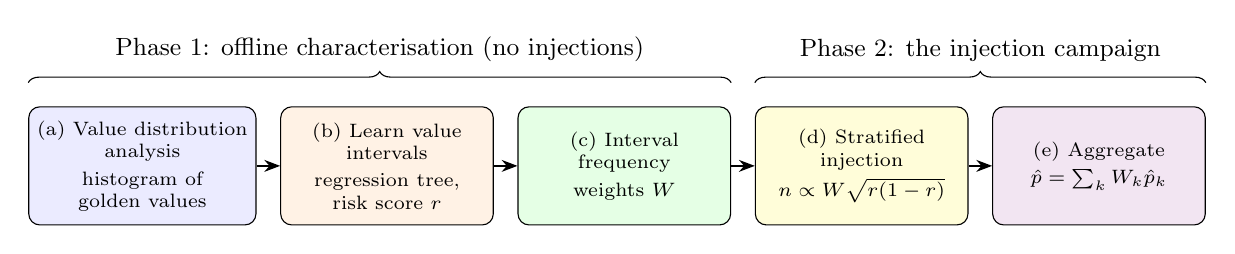
\begin{tikzpicture}[font=\scriptsize, node distance=3mm,
  box/.style={draw, rounded corners, align=center, minimum width=2.7cm, minimum height=1.5cm, inner sep=3pt},
  arr/.style={-{Stealth[length=2mm]}, thick}]
  \node[box, fill=blue!8] (a) {(a) Value distribution\\analysis\\[2pt]histogram of\\golden values};
  \node[box, fill=orange!10, right=of a] (b) {(b) Learn value\\intervals\\[2pt]regression tree,\\risk score $r$};
  \node[box, fill=green!10, right=of b] (c) {(c) Interval\\frequency\\[2pt]weights $W$};
  \node[box, fill=yellow!15, right=of c] (d) {(d) Stratified\\injection\\[2pt]$n\propto W\sqrt{r(1-r)}$};
  \node[box, fill=violet!10, right=of d] (e) {(e) Aggregate\\[2pt]$\hat p=\sum_k W_k\hat p_k$};
  \draw[arr] (a)--(b); \draw[arr] (b)--(c); \draw[arr] (c)--(d); \draw[arr] (d)--(e);
  \draw[decorate,decoration={brace,amplitude=4pt}] ([yshift=3mm]a.north west) -- ([yshift=3mm]c.north east)
     node[midway,above=4pt]{\small Phase 1: offline characterisation (no injections)};
  \draw[decorate,decoration={brace,amplitude=4pt}] ([yshift=3mm]d.north west) -- ([yshift=3mm]e.north east)
     node[midway,above=4pt]{\small Phase 2: the injection campaign};
\end{tikzpicture}
\captionof{figure}{The TreeFI workflow (the paper's Figure~1, redrawn).}
\end{center}

\subsection{Phase 1(a): value distribution analysis}
For each target layer, run the network once, fault-free (the \emph{golden} execution), and build a histogram of the values in that layer. For \emph{activations} this means running the validation set and recording
the layer's outputs; for \emph{weights} the values are read directly from the model parameters.

Two practical points the paper stresses. First, no subsampling: all tensor values are accumulated. Second, to keep this cheap the method stores only \emph{weighted histogram counts} and discards the raw values; values that differ
by less than $10^{-4}$ share a bin. The authors say this reproduces \emph{identical} intervals to those from raw values, and that sorting raw values on large models can take more than a day, versus a few seconds with histograms.

\subsection{Phase 1(b): learning value intervals}
This is the heart of the method. For each \emph{(layer, bit position)} pair a one-dimensional \term{regression tree} is trained along the value axis. A regression tree is a model that repeatedly splits the axis
at the points where the quantity being predicted changes most, ending in ``leaves'', each leaf being an interval of values.

\textbf{What the tree predicts.} Only \emph{how much the value itself changes when that bit is flipped}. In the paper's words, TreeFI ``does not yet perform full inferences through the DNN or evaluate the effect on the model output''. It uses the
numerical difference between the original value and the bit-flipped value, nothing about the network.

\textbf{Settings.} Minimum leaf weight 10 samples, at most 100 leaf nodes, weighted-MSE split threshold $10^{-4}$. In practice the learned trees have at most about 15 leaves per layer-bit pair. Training is weighted by the histogram counts so that rare bins do not distort the splits.

\textbf{From intervals to a risk score.} For each learned interval $k$ of layer $\ell$ and bit $b$, TreeFI averages a \emph{severity}, the log-distance between each original value and its flipped counterpart, giving $\mathrm{avg\_log}_{\ell,b,k}$.
This is turned into a \term{risk score} between 0 and 1 by a sigmoid:
\begin{equation}\label{eq:risk}
r_{\ell,b,k}=\sigma\bigl(s\,(\mathrm{avg\_log}_{\ell,b,k}-\beta_\ell)\bigr),\qquad \beta_\ell=\log_{10}(\gamma\cdot a_{\ell,\max}).
\end{equation}
Here $\sigma(x)=1/(1+e^{-x})$; $s$ controls how sharp the transition is (the paper fixes $s=2$ for all layers); $a_{\ell,\max}$ is the largest golden value in the layer; $\gamma$ is a scaling constant
(they test $1,2,5,10$). In words: intervals where a flip changes the value a lot get a risk close to 1; intervals where it changes the value little get a risk close to 0; the layer-dependent bias $\beta_\ell$ decides what ``a lot'' means relative to the layer's own scale.

\subsection{Phase 1(c): interval frequency}
Using the histogram from (a), compute how often each interval actually occurs in the golden run: the weight $W_{\ell,b,k}$ (the interval's frequency for the layer-bit pair). These weights play two roles: they decide how many injections an interval gets, and they are used to recombine the results.

\subsection{Phase 2(d): stratified injection}
Now the budget is divided across intervals using the classical stratified-sampling rule (Neyman, 1934, the paper's reference 31):
\begin{equation}\label{eq:alloc}
n_{\ell,b,k}\;\propto\;W_{\ell,b,k}\,\sqrt{r_{\ell,b,k}\,(1-r_{\ell,b,k})}.
\end{equation}
Read it as: \emph{more injections for intervals that are frequent (large $W$) and uncertain (risk near 0.5, where $r(1-r)$ is largest).} Intervals with risk near 0 or 1 are nearly certain, so they need few injections. The total per layer-bit pair is chosen
so that the final failure-rate estimate meets the desired confidence and error margin.

\begin{worked}[Illustrative example (numbers invented by me, to show the arithmetic)]
Suppose one layer-bit pair has three intervals:
\begin{center}\small
\begin{tabular}{lccccc}
\toprule
interval & frequency $W$ & risk $r$ & $\sqrt{r(1-r)}$ & $W\sqrt{r(1-r)}$ & share of budget \\
\midrule
1 (small values) & 0.60 & 0.02 & 0.14 & 0.084 & 31.8\% \\
2 (middle) & 0.30 & 0.50 & 0.50 & 0.150 & 56.8\% \\
3 (large values) & 0.10 & 0.90 & 0.30 & 0.030 & 11.4\% \\
\bottomrule
\end{tabular}
\end{center}
With a budget of 1{,}000 injections, uniform-by-frequency sampling would give 600/300/100. The rule above gives about 318/568/114: it takes injections away from the very common but very predictable interval 1 and
puts them where the outcome is genuinely uncertain. After injecting, suppose the measured failure rates in the three intervals are 0.03, 0.48 and 0.88. The estimate is then
\[
\hat p=\sum_k W_k\hat p_k=0.6\times0.03+0.3\times0.48+0.1\times0.88=0.250,
\]
weighted by how common each interval really is.
\end{worked}

\subsection{Phase 2: how the injection is carried out}
\begin{itemize}
\item \textbf{Activation faults.} Activation values depend on the input. For each input, TreeFI looks for activation values whose golden value lies in the chosen interval, picks one location at random among these candidates, and flips the chosen bit. So an activation location is eligible only if
 its value, for the current input, belongs to the interval selected for sampling.
\item \textbf{Weight faults.} The weight value is stored in the parameters and does not depend on the input. TreeFI picks a parameter whose value falls in the interval and flips the chosen bit; the same corrupted parameter can then be evaluated on all the considered inputs.
\item \textbf{Fault model.} A single-bit flip in FP32. The paper chooses this because it is standard in software-implemented reliability studies and gives a simple, controlled setting; it says that real hardware faults may be multi-bit or correlated, but modelling those is out of scope.
\item \textbf{Failure.} The faulty output is compared with the fault-free output and a failure is recorded if the top-1 prediction changes.
\end{itemize}

\subsection{Phase 2(e): aggregating the outcomes}
The failure rate for one layer and bit is the frequency-weighted sum of the interval failure rates:
\begin{equation}\label{eq:agg}
\hat p_{\ell,b}=\sum_k W_{\ell,b,k}\,\hat p_{\ell,b,k}.
\end{equation}
The paper explains why the weighting matters: without it, intervals that are injected often (because they are uncertain) would contribute equally to the estimate even if they rarely occur. Weighting by empirical frequency makes the estimate representative of the actual layer behaviour,
and the paper lists this as one of the main differences from SFI methods that do not distinguish value ranges.

\section{Experimental set-up}
\markboth{TreeFI: set-up}{TreeFI: set-up}

\begin{center}
\small
\begin{tabular}{@{}lp{11cm}@{}}
\toprule
Models & ResNet8 and RepVGG-A0 on CIFAR-10 (trained on the 50{,}000-image training split; injections evaluated on the separate 10{,}000-image test split); DeiT-Tiny, DeiT-Small and DeiT-Base on ImageNet, using ImageNet-pretrained checkpoints and the ImageNet validation set \\
Fault model & FP32 single-bit flips, in activations and in weights \\
Target & absolute error margin $E=1\%$ at $99\%$ confidence \\
Baselines & SFI (data-aware one-shot) and IFI (iterative); IFI starts from a looser target ($E=5\%$) and refines to $1\%$ as recommended \\
TreeFI settings & activations: $\gamma\in\{1,2,5,10\}$ (``TreeFI-$1\times$ \ldots $10\times$'') with $s=2$; weights: TreeFI-$20\times$ \\
Ground truth & exhaustive activation FI on ResNet8, over 5{,}000 inputs \\
Repetition & 15 independent TreeFI campaigns with different random seeds on ResNet8 activations, to measure estimation error and its variability \\
Metric & mean absolute error (MAE) of the failure rate against the exhaustive reference, in percentage points; number of injections; wall-clock time \\
Hardware & one NVIDIA H100 GPU with 96 GB of memory \\
\bottomrule
\end{tabular}
\end{center}
The ``TreeFI-$10\times$'' naming means $\gamma=10$. My reading of equation~(\ref{eq:risk}) (not a sentence from the paper): a larger $\gamma$ raises the bias $\beta_\ell$, which lowers the risk score of every interval, so fewer intervals count as risky and the allocation shrinks.

\section{The results}
\markboth{TreeFI: results}{TreeFI: results}

\subsection{Activation faults on ResNet8, checked against exhaustive FI}
Using the exhaustive campaign as ground truth, TreeFI-$10\times$ gets failure rates very close to the exhaustive ones, reproducing \emph{the same most failure-prone bits and layers}. The paper concludes the reduction in injections
``does not come from overlooking sensitive cases, but from distributing injections more effectively across the value space''.

MAE against the exhaustive reference is below the $1\%$ target for all methods; TreeFI achieves lower MAE than SFI and IFI especially around the most failure-prone layers and bits (the paper's Figure~3). It also has lower per-layer MAE because it combines interval-level results using the
\emph{true interval frequencies} observed in the golden pass; SFI and IFI do not reweight in this way. The gap between TreeFI-$1\times$ and TreeFI-$10\times$ stays below $0.05$ percentage points across layers and bits, one order of magnitude below the $1\%$ target.

\subsection{How many injections? (the paper's Table 1)}
\begin{center}
\small
\begin{tabular}{lrrrrr}
\toprule
method & ResNet8 & RepVGG-A0 & DeiT-Tiny & DeiT-Small & DeiT-Base \\
\midrule
Exhaustive & 9{,}437{,}184 & 14{,}024{,}704 & 58{,}097{,}664 & 116{,}195{,}328 & 232{,}390{,}656 \\
SFI & 740{,}354 & 1{,}812{,}919 & 1{,}664{,}695 & 1{,}749{,}489 & 1{,}781{,}928 \\
IFI & 979{,}021 & 2{,}173{,}770 & n/a & n/a & n/a \\
TreeFI $1\times$ & 100{,}046 & 308{,}303 & 137{,}091 & 113{,}820 & 121{,}702 \\
TreeFI $2\times$ & 76{,}810 & 227{,}601 & 100{,}891 & 77{,}458 & 84{,}379 \\
TreeFI $5\times$ & 49{,}840 & 145{,}525 & 57{,}519 & 41{,}291 & 45{,}672 \\
TreeFI $10\times$ & \textbf{34{,}934} & \textbf{103{,}552} & \textbf{34{,}816} & \textbf{24{,}254} & \textbf{26{,}970} \\
\bottomrule
\end{tabular}
\end{center}
Exhaustive FI needs about $270\times$ more injections than TreeFI-$10\times$ on ResNet8. IFI is not run for the DeiT models because its iterative nature makes the total number of injections impossible to predict and a full-model run is intractable in the authors' set-up.

\textbf{Reduction versus SFI} (the paper's Figure~4): from $5.9\times$ (RepVGG-A0, $\gamma=1$) up to $\mathbf{72.1\times}$ (DeiT-Small, $\gamma=10$). On average TreeFI-$10\times$ reaches the same statistical result as SFI with $44.9\times$ fewer injections.
The gains grow with model size, which the authors read as evidence that the benefit grows with the size of the fault space and the heterogeneity of the value distributions.

\subsection{Time}
\begin{center}
\small
\begin{tabular}{lcc}
\toprule
ResNet8 activations & injections & wall-clock \\
\midrule
SFI & 740{,}354 & 7 h 13 min \\
IFI & 979{,}021 & 9 h 35 min \\
TreeFI-$10\times$ & 34{,}934 & 28 min \\
\bottomrule
\end{tabular}
\end{center}
That is a theoretical reduction of about $21.2\times$ versus SFI and $28.0\times$ versus IFI, and a measured wall-clock reduction of $15.5\times$ and $20.5\times$. On RepVGG-A0 (full activation campaign on the H100): IFI 33 h 47 min, SFI 26 h 46 min,
TreeFI-$10\times$ 1 h 41 min, about $20.1\times$ and $15.9\times$ faster. On the first layer of DeiT-Tiny: IFI 36 h 43 min, SFI 40 h 55 min, TreeFI-$10\times$ 20 min; TreeFI-$10\times$ needed 1{,}042 injections against 124{,}089 (IFI) and 139{,}778 (SFI), about $119\times$ and $134\times$ fewer.
A full DeiT-Tiny analysis with TreeFI-$10\times$ took 6 h 42 min, while SFI needed 111 h 30 min just to complete the first three layers.

\subsection{Scalability on RepVGG and DeiT}
Where exhaustive FI is infeasible the paper compares per-layer and per-bit failure-rate trends (its Figures~5 and 6). TreeFI-$10\times$ follows the same main trends as IFI and SFI with far fewer injections. The small differences it reports in absolute failure rates on DeiT come mainly from the \emph{reweighting step}:
when the authors applied the same reweighting to the SFI results, they obtained estimates matching those of TreeFI-$10\times$.

\subsection{The hyperparameter study (ResNet8 activations)}
To justify the sigmoid parameters, the authors tried $88$ combinations of sharpness $s\in\{1,2,3,4,6,8,16,32\}$ and bias multiplier $\gamma\in\{1,2,5,10,20,50,200,2000,10000,20000,50000\}$. They kept configurations that stayed within the $1\%$ layer-by-bit error criterion:
$60$ of $88$ did. The pattern: for $s\ge16$ only three biases passed, so very sharp transitions concentrate the injections too narrowly and degrade quality; for all $s\le3$ every bias passed. So $s$ matters more than $\gamma$, and they recommend starting from moderate sharpness ($s=2$) and only increasing selectivity if preliminary
experiments justify it. The chosen setting ($s=2$, $\gamma=10$) sits in a conservative part of the trade-off curve (their Figure~7).

\subsection{Weight faults}
Weights do not depend on the input, so there is less structure to exploit. The paper runs all layers of ResNet8, 10 layers of RepVGG-A0 and 6 layers of DeiT-Tiny with TreeFI-$20\times$.
\begin{center}
\small
\begin{tabular}{lrrr}
\toprule
injections (weights) & ResNet8 (all layers) & RepVGG-A0 (10 layers) & DeiT-Tiny (6 layers) \\
\midrule
SFI & 753{,}050 & 1{,}108{,}540 & 310{,}446 \\
IFI & 1{,}043{,}629 & 1{,}560{,}584 & 694{,}557 \\
TreeFI-$20\times$ & \textbf{79{,}426} & \textbf{62{,}063} & \textbf{48{,}465} \\
reduction vs SFI / IFI & $9.5\times$ / $13.1\times$ & $17.9\times$ / $25.1\times$ & $6.4\times$ / $14.3\times$ \\
\bottomrule
\end{tabular}
\end{center}
Run times: ResNet8 1 h 30 (TreeFI) against 14 h 34 (SFI) and 20 h 06 (IFI); RepVGG-A0 1 h 55 against 34 h 27 and 49 h 03; DeiT-Tiny 15 h 46 against 110 h 55 and 227 h 27. The largest difference between the TreeFI estimate and the baselines' is $0.0437$ percentage points (RepVGG-A0, all bits, against IFI),
more than $20\times$ smaller than the $1\%$ target. Reductions for weights are smaller than for activations, as expected: ``weight values vary less, leaving less structure for TreeFI to exploit''.

\section{What the authors conclude, and what they leave open}
\markboth{TreeFI: conclusions}{TreeFI: conclusions}

\textbf{Conclusions.} TreeFI partitions the value distribution into intervals, derives an interval risk score from the severity of bit flips within each interval, and uses it to allocate injections; the final reliability estimate is computed from the measured outcomes. It reduces the injections needed
compared with state-of-the-art SFI while keeping the error within the target margin and preserving the main per-layer and per-bit trends. It is especially attractive for large-scale studies where exhaustive evaluation is infeasible.

\textbf{What they explicitly leave for the future.} The experiments use FP32 single-bit flips. The authors state that the method only requires a fault model that defines how a bit flip modifies a value together with a value distribution that can be collected and partitioned into intervals, so the same interval-learning and
stratified-allocation principle could extend to other numerical formats such as \textbf{FP16, bfloat16 or integer}; ``validating this experimentally is an important direction for future work''. Multi-bit and spatially correlated faults are out of scope.

\textbf{Reproducibility.} The code and artifacts are at \code{gitlab.inria.fr/nbires/treefi}; the paper's repository gives ready-to-run activation and weight examples. The work was supported by the French government (France 2030, PEPR Intelligence Artificielle, project AdaptING, ANR-23-PEIA-0009) and computing from SLICES-FR/Inria.

\section{How TreeFI relates to your project}
\markboth{TreeFI vs your project}{TreeFI vs your project}
\emph{This section is my comparison; the facts about TreeFI above are from the paper and the facts about your project are from your repository.}

\subsection{What you took from it}
\begin{itemize}
\item \textbf{The framing.} Your proposal says ``value-aware stratified sampling (in the spirit of TreeFI, ICCAD 2026) is used as a supporting tool''; your report cites TreeFI as prior work.
\item \textbf{The allocation rule.} $n\propto W\sqrt{r(1-r)}$ is TreeFI's equation~(\ref{eq:alloc}); your MX-TreeFI draft multiplies it by a blast-radius weight $\Phi$. Your \code{neyman_allocation()} implements the rule with and without $\Phi$.
\item \textbf{The model families.} TreeFI used ResNet8, RepVGG-A0 and DeiT-Tiny/Small/Base; your proposal used ResNet8 and RepVGG-A0 on CIFAR-10 and DeiT-Tiny/Small on ImageNet.
\item \textbf{Exhaustive ground truth on ResNet8.} TreeFI did this for activations (9.4 million faults, 5{,}000 inputs); you did it for weights (638{,}624 and 483{,}904 faults, 200 images).
\item \textbf{The 72$\times$ figure.} The ``up to 72$\times$'' in your MX-TreeFI draft is TreeFI's.
\end{itemize}

\subsection{Where your project differs}
\begin{center}
\small
\begin{tabularx}{\linewidth}{@{}l>{\raggedright\arraybackslash}X>{\raggedright\arraybackslash}X@{}}
\toprule
 & TreeFI (the paper) & Your project \\
\midrule
Number format & FP32, each value a self-contained 32-bit word & MX: 4--8-bit elements plus a shared 8-bit scale \\
Fault sites & one: the value & two: element (1 value) and shared scale ($K$ values) \\
What is the goal & fewer injections for a target statistical accuracy & characterise \emph{which formats, bits, layers, tensors} are vulnerable and \emph{why}; sampling is only a supporting tool \\
Failure metric & top-1 prediction change & per-inference rate (and the older any-image rate), plus non-finite rate \\
Impact characterisation & regression tree on the \emph{value change}, no network evaluation, then sigmoid risk score & exact enumeration of the code table; a gradient-based \texttt{margin\_shift} score \\
Tensors & activations and weights & weights (main) and activations \\
Models & ResNet8, RepVGG-A0, DeiT-T/S/B (ImageNet, pretrained) & ResNet8, RepVGG-A0, small ViT (CIFAR-10/100, trained by you) \\
Validation & exhaustive FI on ResNet8 activations & exhaustive FI on ResNet8 weights, two formats \\
\bottomrule
\end{tabularx}
\end{center}

\begin{careful}[A point to check before your viva: what ``learned intervals'' means]
In your E22 experiment and in the report you describe the TreeFI approach as learning value intervals \emph{from a pilot of injected faults} (a regression tree is fitted to each fault's measured network impact), and you found that
this never beat uniform sampling ($0.10$ to $0.98\times$). The README says ``learning value intervals from a pilot run, the way TreeFI does''.

Reading the TreeFI paper (Section~3.3(b)), the tree is trained on \emph{how much the value itself changes under a flip}, ``without evaluating the effect on the model output'', and the risk score comes from the sigmoid of that value change. There is no pilot of injections in the interval-learning step.
So your E22 ``learned tree'' arm tests a pilot-trained variant, which is a legitimate and informative experiment, but it is not necessarily the same as TreeFI as published. A faithful arm would build intervals from the log-distance severity alone.

I have not run that experiment, so I cannot say what it would show. It is possible, from your own finding F3 (the proposal's log-distance severity scores sign flips as zero), that it would struggle on MX weights; TreeFI's FP32 activation plots show the sign bit with a very low failure rate, so the two settings may genuinely differ. That is my inference, not a statement from either document.
Safer wording for the report and README: ``an interval-learning approach in the style of TreeFI, trained on a pilot''. Confirm with your supervisor.
\end{careful}

\subsection{Why your project is a natural next step for the paper}
TreeFI's own future-work paragraph names other number formats as an open direction. MX is such a format, with a feature TreeFI never had to consider (a shared scale with blast radius $K$) and a code space small enough to enumerate exactly. Your E22 result,
that exact enumeration of the code table beats interval learning by about $50\times$ on MX, is a statement about \emph{why the FP32 solution does not carry over unchanged}: TreeFI needs learned intervals because an FP32 alphabet has $2^{32}$ values, and MX does not have that problem.

\part{The project: design and method}

\section{The starting point: your proposal}
\markboth{The proposal}{The proposal}

\subsection{Two drafts, one project}
In August 2026 you wrote two working drafts, both in \code{papers/}:
\begin{enumerate}
\item \emph{Reliability-Aware Fault Injection for Microscaling-Based DNNs: Problem Statement, Fault Model \& Study Design}. A
 \textbf{characterisation} study: how reliable are MX-based networks and why?
\item \emph{MX-TreeFI: Value-Aware Statistical Fault Injection for Microscaling (MXFP) Neural Networks}. A \textbf{method} paper: extend TreeFI from FP32 to MX.
\end{enumerate}
On 10 September you settled which one the project is: \textbf{the first}. MX-TreeFI was kept as reference only. The proposal says so itself, in a box: \emph{``TreeFI-style value-aware stratified sampling is referenced only to make the multi-axis campaign affordable.
The contribution of this work is the reliability characterization of microscaling DNNs, not a faster injection method.''}

\subsection{The core hypothesis and the five objectives}
\begin{keyidea}
\textbf{Core hypothesis.} Reliability of microscaling DNNs varies substantially across formats \emph{even at comparable inference accuracy}, and faults in the shared scale behave very differently from faults in individual elements, because a single scale fault rescales an entire block of $K$ values at once.
\end{keyidea}
\begin{description}[leftmargin=1.2cm,style=nextline]
\item[O1 Fault propagation] How do single-bit faults in elements versus shared scales propagate, and how big is the difference?
\item[O2 Format sensitivity] Measure sensitivity across MXFP8/6/4 and element variants; test whether reliability differs at comparable accuracy.
\item[O3 Block-size effect] How does the scale-sharing granularity trade efficiency against reliability?
\item[O4 Tensor and location] Compare weights versus activations, and fault locations (scale bit versus element bit, MSB versus LSB, per layer).
\item[O5 Vulnerability drivers] Which representation characteristics (dynamic range, exponent/mantissa split, scale granularity) explain the observed vulnerability?
\end{description}

\subsection{The fault model in the proposal, symbol by symbol}
The proposal separates fault \emph{occurrence} (where and how often bits flip) from fault \emph{impact} (how much the decoded value changes).

\textbf{Impact.} For an element flip of bit $b$ the proposal defines the severity
\[
d=\bigl|\log v'-\log v\bigr|,
\]
the distance on a logarithmic scale between the new and old value (affects 1 value). For a scale flip, every value in the block becomes $v'_{i,s}=m_{i,s}\,2^{X'-\mathrm{bias}}$ and the \emph{block severity} is
\[
D_s=\sum_i\bigl|\log v'-\log v\bigr|=K\cdot|X'-X|\cdot\log2 .
\]
In words: a scale flip rescales the whole block by $2^{X'-X}$, so the damage is $K$ times a single-value log change.

\textbf{Occurrence.} Each bit position $b$ of a site has a flip probability $\pi_{\mathrm{site},b}=\pi^{0}_{\mathrm{site}}\,\kappa_{\mathrm{site}}(b)$: a base rate times a position profile $\kappa(b)$ whose average is 1. $\kappa\equiv1$ gives the uniform single-bit model (every bit equally likely). Since bits flip independently,
the probability of a specific flip pattern $S$ is the \emph{Poisson-binomial} expression
\[
P(S)=\prod_{b\in S}\pi_b\prod_{b\notin S}(1-\pi_b),
\qquad
H_{\mathrm{site}}=1-\prod_b(1-\pi_b)\approx\sum_b\pi_b+\sum_{b<b'}\pi_b\pi_{b'}+O(\pi^3).
\]
$H$ is the probability that a word is corrupted at all. The first term is the single-bit contribution; the second is the multi-bit tail, the proposal's ``H-model''. Your project settled whether that tail needs its own campaign (it does not; Section~\ref{sec:multibit}).

\subsection{The study design table}
\begin{center}
\small
\begin{tabular}{@{}lp{11.5cm}@{}}
\toprule
Format & MXFP8 (E4M3, E5M2), MXFP6 (E3M2, E2M3), MXFP4 (E2M1); optional MXINT8. Shared scale E8M0. \\
Block size & 8 / 16 / 32 / 64 (fewer values per scale means a smaller blast radius) \\
Tensor type & weights (input-independent) and activations (input-dependent) \\
Fault location & scale bit versus element bit; MSB to LSB within each field; per-layer position \\
Models & ResNet8, RepVGG-A0 (CIFAR-10); DeiT-Tiny/Small (ImageNet); optional small LLM \\
Fault model & single-bit flip at both sites; multi-bit (H-model) as an extension \\
Metrics & top-1 change / accuracy drop; per-site failure and SDC rate; per-bit and per-layer maps \\
\bottomrule
\end{tabular}
\end{center}

\subsection{The methodology the proposal prescribes}
\begin{description}[leftmargin=1.2cm,style=nextline]
\item[Quantization] Quantize weights and activations to each MX configuration; confirm baseline accuracy so reliability is compared at matched accuracy.
\item[Injection engine] A bit-addressable MX representation: faults at a chosen bit of the scale or of an element; weights are static, activations are injected per input through hooks; golden-versus-faulty comparison detects top-1 changes and SDC.
\item[Campaign] For each cell of the study matrix, run a statistical FI campaign at a target confidence; value-aware stratified sampling in the spirit of TreeFI is a supporting tool.
\item[Ground truth] Exhaustive FI on a small model (ResNet8) to validate the statistical estimates.
\item[Analysis] Compare sensitivity across the four axes; contrast scale versus element faults; correlate vulnerability with representation characteristics to explain trends.
\end{description}

\subsection{Expected outcomes and open choices}
The proposal expected: shared-scale faults with significantly larger impact; reliability varying across formats at equal accuracy; a block-size trade-off; per-tensor and per-location maps of what needs protection; and design guidance. It listed three open design choices, \emph{settled empirically}: learned versus exact interval characterisation; single-bit versus multi-bit; and the block-size/format grid actually swept, bounded by compute.

\section{The tool: \code{mxfi}}
\markboth{The tool mxfi}{The tool mxfi}

\subsection{Architecture}
\begin{center}
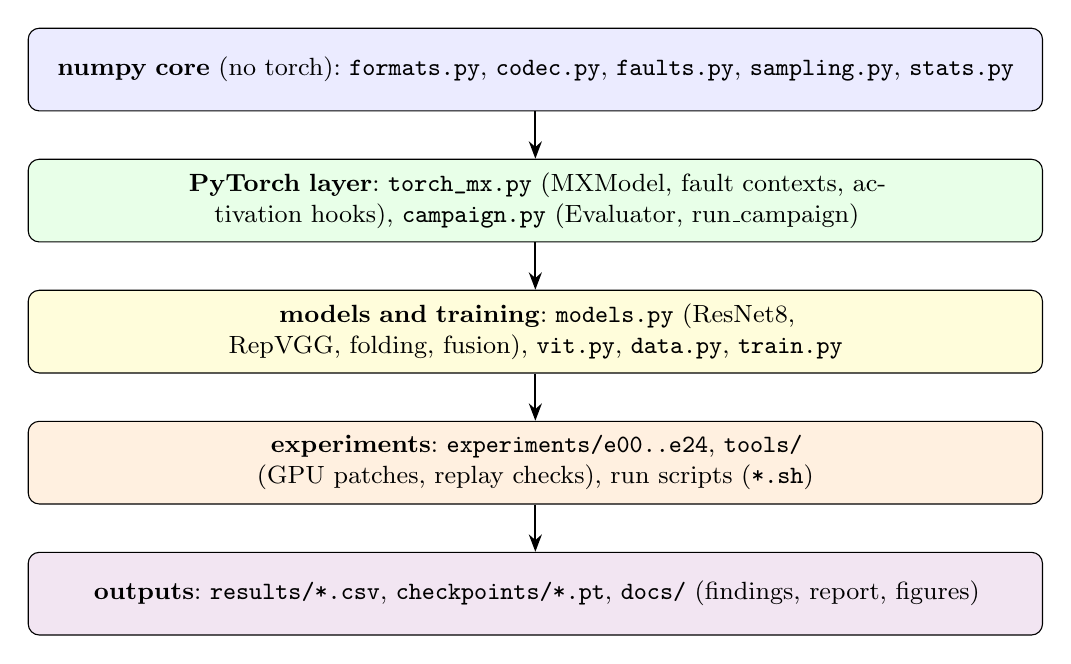
\begin{tikzpicture}[font=\small, node distance=6mm,
  layer/.style={draw, rounded corners, text width=12.6cm, minimum height=1.05cm, align=center, inner sep=4pt},
  arr/.style={-{Stealth[length=2.2mm]}, thick}]
  \node[layer, fill=blue!8] (core) {\textbf{numpy core} (no torch):\ \code{formats.py}, \code{codec.py}, \code{faults.py}, \code{sampling.py}, \code{stats.py}};
  \node[layer, fill=green!9, below=of core] (torch) {\textbf{PyTorch layer}:\ \code{torch_mx.py} (MXModel, fault contexts, activation hooks), \code{campaign.py} (Evaluator, run\_campaign)};
  \node[layer, fill=yellow!14, below=of torch] (models) {\textbf{models and training}:\ \code{models.py} (ResNet8, RepVGG, folding, fusion), \code{vit.py}, \code{data.py}, \code{train.py}};
  \node[layer, fill=orange!12, below=of models] (exp) {\textbf{experiments}:\ \code{experiments/e00..e24}, \code{tools/} (GPU patches, replay checks), run scripts (\code{*.sh})};
  \node[layer, fill=violet!10, below=of exp] (out) {\textbf{outputs}:\ \code{results/*.csv}, \code{checkpoints/*.pt}, \code{docs/} (findings, report, figures)};
  \draw[arr] (core)--(torch); \draw[arr] (torch)--(models); \draw[arr] (models)--(exp); \draw[arr] (exp)--(out);
\end{tikzpicture}
\captionof{figure}{How the pieces of the repository fit together. The bottom of the stack uses everything above it.}
\end{center}
The core is pure numpy so the representation-level analysis (formats, codec, fault tables, sampling, statistics) runs anywhere; only \code{torch_mx.py} imports torch.

\subsection{\code{formats.py}: the exact alphabets}
Defines an \code{ElementFormat} (exponent bits, mantissa bits, has\_inf, has\_nan) and builds an \emph{exact lookup table over every possible code}. Because the alphabets are tiny (16 to 256 codes), the table is both the decoder and the ``exact enumeration'' used later for analysis.
Handles subnormals, e4m3's convention (only the all-ones mantissa at the top exponent is NaN) and e5m2's IEEE-style specials (mantissa 0 is Inf, anything else is NaN). Also the E8M0 scale encode/decode, with code 255 as NaN, computed in float64 so $2^{127}$ cannot overflow before conversion. Aliases such as \code{mxfp8}, \code{mxfp6}, \code{mxfp4} are accepted.

\subsection{\code{codec.py}: bit-addressable encoding}
\code{quantize()} turns a float tensor into an \code{MXTensor} holding two separately addressable \code{uint8} arrays: \code{scales[..., n_blocks]} (site X, 8 bits each) and \code{codes[..., n_blocks, block_size]} (site r, $w$ bits each). Steps inside:
\begin{enumerate}
\item move the blocking axis to the end and pad the last block with zeros if needed (padding lanes are marked invalid and never injected);
\item compute the block maximum, then the scale by the OCP or fit rule; all-zero blocks get scale exponent 0;
\item \textbf{if any element of a block is NaN, the block's scale is set to the NaN code 255} (the fix you made on 2 October; see Section~\ref{sec:phase-c100});
\item divide by the scale, round to the nearest representable magnitude (ties to even) and saturate at the largest value, then set the sign bit.
\end{enumerate}
\code{decode()} reverses this; a faulted scale can reach $2^{127}$ and the product legitimately overflows to infinity, so that warning is suppressed on purpose.

\subsection{\code{faults.py}: injecting and enumerating}
\code{Fault(site, index, bit)} names a flip; \code{inject()} XORs one bit on a \emph{copy}. \code{fault_space()} counts addressable bits per site (padding excluded). The two impact tables enumerate \textbf{every (code, bit) and every (scale byte, bit)} flip in closed form:
\begin{itemize}
\item \code{element_impact_table(fmt)}: before and after values, \code{log_severity} (the proposal's metric), \code{rel_error}, a sign-flip mask, and whether the flip goes to or comes from NaN/Inf.
\item \code{scale_impact_table()}: for every byte and bit, the exponent change $\pm2^{\mathrm{bit}}$, the multiplier, whether the flip reaches the NaN byte, and whether it overflows float32. Exactly eight bytes flip into the NaN scale (a test pins this).
\end{itemize}
A comment in the file already records the finding that the proposal's severity is blind to the sign bit.

\subsection{\code{sampling.py} and \code{stats.py}}
\code{sample_uniform} draws every stored bit with equal probability (a multinomial over (tensor, site) strata weighted by bit counts, then a uniform slot and bit inside); \code{sample_stratified} draws a requested number from each stratum and returns \emph{inclusion weights}
(stratum share divided by draws) so a weighted mean stays unbiased. \code{neyman_allocation} implements $W\sqrt{r(1-r)}\,\Phi$ with a floor, using largest-remainder rounding; \code{default_blast_weight} sets $\Phi=K$ for scale strata. In \code{stats.py}: Wilson intervals, the stratified estimator and its variance,
\code{required_samples}, and \code{injection_reduction} (the ``$N\times$ fewer injections'' figure).

\subsection{\code{torch_mx.py}: putting MX inside a PyTorch model}
\code{MXModel} wraps a model without copying it.
\begin{itemize}
\item \textbf{Blocking follows the reduction axis}, as hardware reads a tensor: a \code{Linear} weight $(\text{out},\text{in})$ is blocked along \code{in}; a \code{Conv2d} weight $(\text{out},\text{in},k_h,k_w)$ is viewed as $(\text{out},\text{in}\cdot k_h k_w)$ and blocked along that flattened axis.
\item \code{quantize_weights()} encodes every target layer, stores the pristine FP32 weights and the \code{MXTensor}, and writes the decoded values back.
\item \code{fault(site)} is a context manager: it patches only the weights the fault touches (one value for an element fault, up to $K$ for a scale fault), yields, then restores them exactly. \code{word_fault()} does the same for a multi-bit mask confined to one word (used by E21).
\item Activations: forward \emph{pre-hooks} quantise a layer's input to MX (blocks along channels for conv, features for linear), optionally flip one bit of the encoding, and decode before the layer runs; \code{activation_space()} captures the MX form of each layer's input for one batch to define the fault space.
\item \code{MXConfig} holds one cell of the study grid: format, block size, scale mode, whether to quantise weights and/or activations, skip-first/last layer options.
\end{itemize}

\subsection{\code{campaign.py}: the evaluation loop}
\code{Evaluator} materialises the fixed evaluation set into batches once, so every injection replays identical inputs; \code{predict()} returns top-1 predictions and whether any logit was non-finite (a NaN row is marked class $-1$ so it always counts as changed). \code{Golden} stores the fault-free predictions and accuracy.
\code{run_campaign()} injects each fault, scores it, and writes one CSV row. Each row records:
\begin{itemize}
\item \textbf{what was injected}: \code{tensor, site, bit, index};
\item \textbf{what happened}: \code{changed} (number of predictions changed), \code{change_rate}, \code{sdc} (changed $>0$), \code{accuracy}, \code{acc_drop}, \code{nonfinite};
\item \textbf{what the representation predicted}: \code{code, value_before, value_after, log_severity, rel_error, sign_flip, to_nonfinite, blast_radius}, and the inclusion \code{weight}.
\end{itemize}
Carrying the predicted severity next to the observed outcome is what made the severity-versus-failure analysis possible. Recording the \emph{count} \code{changed} per fault, even in the first campaigns, is also what let you rescore everything per inference later without a single new injection.

\subsection{\code{models.py}, \code{vit.py}, \code{data.py}, \code{train.py}}
\begin{itemize}
\item \textbf{Deployment form.} \code{to_deploy()} converts a trained model to what an accelerator would run. For ResNet8 it \emph{folds batch normalisation into the convolution}: with BN scale $g=\gamma/\sqrt{\sigma^2+\varepsilon}$, the folded weights are $W'=W\cdot g$ and bias $b'=(b-\mu)g+\beta$. For RepVGG it \emph{fuses the three branches} into one $3\times3$ convolution (the $1\times1$ kernel is zero-padded to $3\times3$, the identity branch becomes an identity kernel, each is first BN-folded, then kernels and biases are summed, and the block's ReLU is kept).
 Why this matters: an unfolded BatchNorm would renormalise whatever a corrupted convolution produced and hide damage, so measured failure rates would describe a network nobody ships.
\item \textbf{Registry.} \code{MODELS} holds \code{resnet8}, \code{repvgg_a0}, \code{vit_small}, the width variants \code{resnet8_w8..w64}, and \code{_c100} variants with a 100-class head. A \code{_c100} suffix both selects the architecture's 100-class head and the dataset, so checkpoint and result names from CIFAR-10 and CIFAR-100 cannot collide.
\item \textbf{ViT.} Patch embedding by a strided convolution, a class token, learned positional embeddings, 6 pre-norm blocks (LayerNorm, attention with explicit \code{qkv} and \code{proj} \code{Linear} layers, GELU MLP with ratio 4) and a linear head. Written out so the quantiser sees every projection; LayerNorm stays unquantised.
\item \textbf{Data.} CIFAR-10/100 with standard normalisation. \code{campaign_subset} draws a \emph{fixed, class-balanced} subset of the test set (seed 0), materialised in memory: 200 images in every campaign (20 per class on CIFAR-10, 2 per class on CIFAR-100), so per-inference rates have the same resolution everywhere.
\item \textbf{Training.} Resumable (saves every epoch), seed-aware checkpoint names (\code{model_cifar10.pt} for seed 0, \code{model_s1_cifar10.pt} for seed 1, \ldots), optional AdamW, label smoothing, a \code{STOP_FILE} so a long sweep can halt cleanly after the current epoch. On CUDA, TF32 is disabled and cuDNN set deterministic so GPU numbers stay comparable with CPU ones.
\end{itemize}

\subsection{The tests (about 1{,}100 lines)}
\begin{itemize}
\item \code{test_codec.py}: exhaustive checks over the whole code space: alphabet geometry, monotone positive half, known spec values, $e_{\max}$ values, E8M0 round trip, representable values encode exactly, round-to-nearest-even, quantisation is idempotent, scaled blocks land in range, the scale rule matches the OCP formula, headroom values, OCP clips and fit never clips, all-zero blocks,
 shapes and axes, padding, bit accounting, deep copy, and (added after the bug) \emph{a NaN input makes its own block NaN and only its block}.
\item \code{test_faults.py}: injection does not mutate the original; it is an involution; bad sites and bits are rejected; blast radius is 1 for elements and $K$ for scales; the scale fault rescales exactly; fault-space accounting; the sign bit is invisible to the log-severity metric; exponent-bit severity doubles per position; only FP8 can flip into non-finite; exactly eight bytes flip into the NaN scale; the scale MSB is the most damaging bit.
\item \code{test_sampling.py}: population matches storage; padding excluded; uniform sampling hits sites in proportion to bits; Neyman favours uncertain strata; $\Phi$ up-weights the scale stratum; the stratified estimate is unbiased against a known truth; Wilson edge cases; required-sample scaling.
\item \code{test_torch_pipeline.py}: ResNet8 shape and size; BN folding preserves the function and removes every BatchNorm; conv weights are blocked along the reduction axis; restoring weights is exact; the fault context restores the quantised weights; the blast radius shows in the weights; \code{word_fault} matches the whole-tensor path; the campaign is deterministic and side-effect free;
 RepVGG reparameterisation is exact and keeps the ReLU; checkpoint names are seed-aware; CIFAR-100 models are named and sized apart; the ViT geometry and quantisation.
\end{itemize}

\subsection{The tools in \code{tools/}}
\begin{description}[leftmargin=1.2cm,style=nextline]
\item[\code{device_support.py}] An idempotent patch that adds GPU support: batches live on the device, activation hooks return tensors on the model's device, training takes \code{--device}. The MX codec stays on the CPU in numpy (exact and cheap); only forward passes move to the GPU.
\item[\code{fast_inject.py}] An idempotent patch that makes weight injection $O(K)$ instead of $O(\text{parameters})$: before, each injection decoded the whole tensor twice. Measured on an A100, ResNet8-w16 went from 24.6 ms to 8.1 ms per injection and w48 from 31.8 ms to 13.9 ms.
\item[\code{verify_fast_inject.py}] Proves the fast path equals the original over 1{,}290 faults, including padding lanes, the scale MSB and flips onto the NaN scale; also checks weights are restored exactly.
\item[\code{verify_ground_truth.py}, \code{verify_e01.py}] Replay a sample (about 300) of a recorded campaign's faults against a checkpoint and compare outcomes: a matched pair agrees on essentially every fault; a mismatched one lands near 0.67 to 0.85. Born from the checkpoint mismatch of September (Section~\ref{sec:phase-metric}).
\end{description}

\section{Networks, training and campaign protocols}
\markboth{Protocols}{Protocols}

\subsection{Training recipes}
\begin{center}
\small
\begin{tabular}{@{}lp{11cm}@{}}
\toprule
CNNs (ResNet8, RepVGG) & SGD with Nesterov momentum 0.9, learning rate 0.1, weight decay $10^{-4}$, batch 128, cosine learning-rate schedule, cross-entropy, random crop (padding 4) and horizontal flip, per-dataset mean/std normalisation. 60 epochs for the first ResNet8 (87.01\%); 30 epochs for RepVGG-A0 (91.44\%) and for every width-sweep network. \\
ViT & AdamW, learning rate $10^{-3}$, weight decay 0.05, label smoothing 0.1, 100 epochs; 80.4--81.9\% on CIFAR-10 over three seeds. \\
CIFAR-100 & the same recipes unchanged: ResNet8 $\approx58\%$, RepVGG-A0 70--71\%, ViT 47--49\%, three seeds each. \\
Seeds & seed 0 keeps the unsuffixed checkpoint name; seed $s>0$ adds \code{_s<s>}; the ten-seed width sweep used seeds 0--9. \\
\bottomrule
\end{tabular}
\end{center}

\subsection{The weight campaign, step by step}
\begin{enumerate}
\item Train and load the network; convert to deployment form.
\item Quantise every Conv2d/Linear weight tensor to MX (format, $K=32$, OCP rule) and write the decoded values back. Record quantised accuracy (E00).
\item Choose the fixed 200-image class-balanced subset; compute golden predictions.
\item Draw 3{,}000 faults uniformly over every stored bit (elements and scales, all layers; padding excluded); a fixed random seed makes the fault list reproducible.
\item For each fault: apply it (patch the touched weights), run the 200 images, record which and how many predictions changed and whether any logit was non-finite, restore the weights.
\item Write the CSV; summarise with Wilson intervals (any-image) or interval on the mean of \code{change_rate} (per inference).
\end{enumerate}

\subsection{The other protocols}
\begin{description}[leftmargin=1.2cm,style=nextline]
\item[Exhaustive (E06)] Replace the random draw with a fixed enumeration of every (layer, row, block, lane, bit) and every (layer, row, block, scale-bit). Streams to CSV in chunks and is resumable. ResNet8-w16: 638{,}624 faults in e4m3 and 483{,}904 in e3m2.
\item[Activations (E04)] Per-inference protocol: batch of one, the fault injected into that inference's own activation buffer. Activation blocks run down the channel axis and the batch axis is separate, so batch-of-one is the \emph{exact} per-inference fault space, not an approximation. After the codec fix: 100 images, 4{,}000 faults per campaign.
\item[Matched block-size study (E03b)] One fixed set of (layer, weight position, bit) triples injected at every block size, re-mapped as \texttt{(row, col//K, col\%K)}, so only the grouping varies.
\item[Multi-bit (E21)] Sample words (1{,}500 element codes and 500 scale bytes per format), inject every single-bit and every two-bit mask of each; record which images changed as a packed bit string so a double flip can be compared with the union of its two single flips.
\item[Replay studies (E15, E18--E22)] Because the exhaustive campaigns recorded every fault's outcome, any sampling strategy can be replayed against the truth hundreds of times without a further inference.
\end{description}

\subsection{Quality controls built into the work}
Every control exists because something went wrong without it:
\begin{itemize}
\item the exhaustive campaigns validate the sampling (the 3{,}000-fault estimate covered the truth twice);
\item the fast injection path is proven identical to the slow one; GPU and CPU agree on 99.97\% of per-injection outcomes (one borderline case in 3{,}000);
\item E21's single-bit rates reproduce the exhaustive campaign (e3m2 element 0.00103 against 0.00113, scale 0.1875 against 0.1887);
\item E23's sampled NaN-guard estimate matches the exhaustive figure to four significant digits;
\item replay checks tie each campaign to its checkpoint (E15 refuses to continue below 0.98 agreement);
\item a unit test pins the NaN behaviour of the codec.
\end{itemize}

\section{Index of the experiments}
\markboth{Experiment index}{Experiment index}
Each script in \code{experiments/} has a docstring stating the question and how to run it. Numbers in brackets are the finding numbers in \code{docs/findings.md}.

\begin{center}
\footnotesize
\begin{longtable}{@{}p{3.0cm}p{5.0cm}p{7.2cm}@{}}
\toprule
script & question & outcome \\
\midrule
\endhead
e00 & MX-quantised accuracy across the grid; which formats are accuracy-matched? & formats within a fraction of a point at $K=32$, MXFP4 lower; baseline for every rate \\
e01 & uniform 3{,}000-fault baseline per format & the first results; scale faults dominate [F1--F5] \\
e02 & uniform versus Neyman versus Neyman+$\Phi$ at equal budget & unbiased; $\Phi$ gives $10.5\times$ on the scale stratum but widens the model-wide interval [F8--F11] \\
e03, e03b & block size, independent and matched faults & scale side monotone worse with $K$; OCP clipping distorts the any-image trend [F14--F16, F57] \\
e04 & weights versus activations, per inference & scale dominates in both; after the codec fix weights $\approx$ activations per fault [F12, F13, F69] \\
e05c & are any-image SDC rates measuring near-ties? (signflip, margins, robust) & yes; Spearman $+0.89$ with near-tie count [F26] \\
width\_sweep\_* & capacity versus vulnerability, single and multi-seed & dose-response by special-code count [F21--F25, F29--F31] \\
e06 & exhaustive ground truth on ResNet8 & truth 0.4171 (e4m3), 0.1079 (e3m2); sampling validated [F27, F28, F41, F53, F54] \\
e08, e09, e09b & why do e3m2 and e2m3 (both 6-bit) differ $5.8\times$? & not perturbation size, not which weights [F35] \\
e10, e11 & margins; sensitivity $s$ & fragility is a property of the quantised network; $s$ predicts the probe at $+0.998$ [F36--F38] \\
e12 & a severity measure that predicts failure & \code{margin_shift}, AUC 0.990 [F39] \\
e14, e16, e17 & where the sensitivity tail comes from & not marginals, not alignment; it is the hardest image's margin [F44, F48, F49] \\
e15 & value-aware sampling against exhaustive truth & $7.0\times$ (e3m2), $2.3\times$ (e4m3), any-image [F46, F47] \\
e18 & how much of a rate belongs to the evaluation set? & nine image sets: the any-image metric is the confound [F50--F52] \\
e19 & every campaign rescored per inference & ordering holds on 8 of 8 models [F55--F59] \\
e20 & value-aware sampling re-derived per inference & $57$--$120\times$ [F60, F61] \\
e21 & single versus multi-bit & single-bit is sufficient [F62--F64] \\
e22 & learned intervals versus exact enumeration & enumeration $48$--$65\times$; learned $\le1\times$ [F65, F66] \\
e23 & read-side NaN guard & $\ge29\times$ on RepVGG and ViT [F68, F72] \\
e24 & CIFAR-100 as the ImageNet stand-in & everything replicates; gap narrows [F70--F72] \\
compare\_arch\ldots, make\_figures & cross-architecture check; the report's four figures & \\
\bottomrule
\end{longtable}
\end{center}
E07 (the ViT study) has no script of its own: it was run by \code{vit_run.sh}. There is no script named \code{e13}, and the numbering has other gaps; the findings log attributes work to the numbers.

\section{Infrastructure and bookkeeping}
\markboth{Infrastructure}{Infrastructure}

\subsection{The two machines}
\begin{center}
\small
\begin{tabular}{@{}lp{6.2cm}p{6.2cm}@{}}
\toprule
 & Laptop & IITK GPU server \\
\midrule
Hardware & Intel i5-1035G1 (4 cores/8 threads at 1.0 GHz), 11.7 GB RAM, integrated graphics, no CUDA & 2$\times$ NVIDIA A100-PCIE-40GB (often shared with other users), 32 CPU cores, no job scheduler \\
Software & Python 3.13, torch 2.14.0+cpu (\code{.venv}) & Python 3.8.5, torch 2.1.2+cu121, numpy 1.24.3, pandas 1.4.4 \\
Network & slow (about 100 kB/s; CIFAR-10 took about 35 min) & no outbound internet, so no downloads and no ImageNet \\
Space & ample & \code{/home} and \code{/data} 100\% full; work in \code{/data/rajeshr/peeyush/bitflip} \\
Speeds & ResNet8 training 82 s/epoch; 47 ms per injection (100 images) & 8.1 ms (w16) per injection after the patch; 4--10$\times$ the server's 32 cores, 13--30$\times$ the laptop; exhaustive w16 about 1.1--1.4 h \\
\bottomrule
\end{tabular}
\end{center}
Long jobs on the server are launched detached so they survive the SSH session, with the parentheses form \texttt{(nohup env ... python -m experiments.X > log 2>\&1 \&)} so only the python command is backgrounded.

\subsection{Run scripts}
\code{run_repvgg_experiments.sh} waits for RepVGG training then runs E00, E01 and E03b; \code{run_width_sweep.sh} and \code{run_width_sweep_seeds.sh} (seed-first, restartable) run the CPU width sweeps; \code{sweep_lock.sh} and \code{logs_wait_then_sweep.sh} stop two runners starting at once;
\code{gpu_width_sweep.sh} runs ten seeds per width on the A100; \code{remaining_gpu.sh} (RepVGG three seeds, exhaustive e3m2, activations on RepVGG and ViT); \code{vit_run.sh} (ViT three seeds, five formats); \code{c100_run.sh} (CIFAR-100 in two GPU lanes plus an activations lane);
and under \code{cluster/}: \code{e04_rerun.sh}, \code{e21_run.sh}, \code{e22_run.sh}, \code{e23_run.sh}. All are restartable: a trained width is not retrained and a finished campaign is not rerun, and \code{touch logs/STOP} halts them cleanly.

\subsection{Lessons about long jobs on Windows}
\begin{itemize}
\item Stopping a background task does \emph{not} kill its children: in September two runners trained the same checkpoint in lockstep for about 17 hours. A lock file now records the Windows PID (Git Bash's \texttt{\$\$} is an MSYS PID that \code{tasklist} cannot find).
\item Never run a long job inside a monitor; never edit a bash script while it is running (bash reads it incrementally).
\item The laptop sleeps (inflating epoch time from minutes to hours) and Windows Update rebooted it once, killing a run; sleep must be set to never and updates paused by the user.
\end{itemize}

\subsection{Checkpoint provenance}
Training is not bit-reproducible across machines or library versions. Of the 24 checkpoint names that exist both on the laptop and on the cluster, \emph{none} has identical weights, yet accuracies agree within a few tenths of a point, so nothing looks wrong. Result files were copied in both directions, so a result and a checkpoint with the same name could come from different networks.
Consequently the repository keeps the cluster's outputs in \code{cluster/} separately (57 same-named files differ), and the verification scripts exist. Known identities: the laptop's \code{resnet8_w16} is the cluster's \code{resnet8_w16_s9}; the e3m2 exhaustive campaign is cluster train-seed 0 and the e4m3 one is train-seed 9.

\subsection{The repository and its history}
Everything is tracked: code, results, trained weights, the CIFAR datasets (the three files over GitHub's 100 MB limit go through Git LFS), logs, and \code{cluster/}, a verbatim mirror of the server's outputs checked file by file against its MD5 sums (425 checkpoint and result files). Only \code{.venv}, caches, LaTeX intermediates and the live \code{STOP} files are ignored.
Fifteen commits from \emph{Initial commit} (22 September) to \emph{Update report} (5 October), pushed to \code{github.com/peeyushagarwal2004/CS496_UGP}.

\part{The work, in the order it was done}

Each phase below is told the same way: the question you were asking, what you did, what you found, and what it changed. Dates are from your report and findings log.
Where a result was later revised, I say so at the point it first appears, and Section~\ref{sec:mistakes} collects all revisions.

\begin{center}
\small
\begin{tabular}{@{}rp{3.3cm}p{9.7cm}@{}}
\toprule
 & dates (2026) & phase \\
\midrule
1 & 9--11 Sep & Scope, hardware, the tool; first campaigns on ResNet8 \\
2 & 11 Sep & A first attempt at cheaper campaigns (stratified sampling) \\
3 & 11--12 Sep & Weights versus activations; block size \\
4 & 12--13 Sep & A second architecture; the NaN mechanism; first width sweep \\
5 & 17--20 Sep & More seeds; the near-tie puzzle \\
6 & 20--22 Sep & GPU server: exhaustive ground truth, ten seeds, a transformer \\
7 & 22--25 Sep & The 6-bit puzzle, sensitivity, a severity measure that works \\
8 & 25--27 Sep & Two mistakes caught; the change of metric; value-aware sampling re-derived \\
9 & 28 Sep--1 Oct & The proposal's two open design choices settled \\
10 & 1--2 Oct & The read-side NaN guard \\
11 & 2--3 Oct & A bug in your own codec; CIFAR-100 \\
12 & 3--5 Oct & Wrap-up, push, report rewrite \\
\bottomrule
\end{tabular}
\end{center}

% =====================================================================
\section{Phase 1: Scope, hardware, the tool, first campaigns (9--11 Sept)}
\markboth{Phase 1}{Phase 1}

\subsection{What was decided}
\begin{itemize}
\item The project is the characterisation study (decided 10 September; see Part~III). TreeFI-style sampling is a supporting tool only.
\item The dev machine has no CUDA GPU, so ImageNet/DeiT cannot be run locally: one ImageNet validation pass would take about half an hour and a campaign needs thousands. Decision: start at CIFAR scale with ResNet8 and RepVGG-A0, keep the code portable so heavy runs can move to a GPU.
\item You \emph{measured} the cost of an injection: 47 ms on 100 images on four CPU threads (89 ms on 200). At that speed the \emph{entire} e4m3 weight bit space of ResNet8 (638{,}624 faults) is about a 16-hour run. Your first guess had been months, because you had assumed every fault would be scored on all 10{,}000 test images.
 Knowing that exhaustive truth was affordable changed what the project could promise.
\end{itemize}

\subsection{The first network}
ResNet8 trained on CIFAR-10 to \textbf{87.01\%} top-1, matching the MLPerf Tiny reference (82 s per epoch on the laptop).

\subsection{The first campaigns and what they showed}
3{,}000 uniformly sampled weight faults per format, $K=32$, any-image metric, 200-image subset:
\begin{center}
\small
\begin{tabular}{lcccc}
\toprule
format & bits & accuracy & any-image SDC [95\% CI] & non-finite outputs \\
\midrule
e5m2 & 8 & 84.80\% & 28.9\% [27.3, 30.6] & 7.7\% \\
e3m2 & 6 & 84.85\% & 51.3\% [49.5, 53.1] & 0.0\% \\
e4m3 & 8 & 85.08\% & 32.3\% [30.7, 34.0] & -- \\
\bottomrule
\end{tabular}
\end{center}
\begin{enumerate}
\item \textbf{The hypothesis looked right immediately.} e5m2 and e3m2 differ by 0.05 accuracy points but $1.77\times$ in vulnerability, with disjoint intervals (F1). The 6-bit format looked \emph{worse}; that direction was later shown to be a metric artefact, but the larger point, that equal accuracy does not mean equal reliability, survived everything.
\item \textbf{The failure \emph{modes} differ} (F2). e5m2 fails rarely but catastrophically: it has special codes, and 7.7\% of its faults gave NaN/Inf. e3m2 fails often but mildly and never produced a non-finite output. This was the first hint of the central mechanism. Worst e5m2 bit: exponent bit 3 (65.8 images changed, 32.7\% non-finite). Worst e3m2 bit: the sign bit.
\item \textbf{The proposal's severity metric did not work} (F3). Over 8{,}374 element faults the rank correlation of $d=|\log v'-\log v|$ with observed failure was $0.026$. A sign flip leaves $|v|$ unchanged, so $d$ scores it zero, yet the zero-severity bucket had the \emph{highest} failure rate (49.8\%), and the sign bit was the single most damaging bit in e4m3 (52.8\%) and e3m2 (56.1\%).
 A sampler built on $d$ would give the most dangerous bit almost no budget. \code{rel_error} did better (0.231).
\item \textbf{Scale faults dominated} (F4, F5). Scale faults were 2--3$\times$ more likely than element faults to change a prediction (e4m3: 30.3\% element against 91.8\% scale), changed 37--41 of 200 predictions on average against 0.7--15.6 for elements, and 9--13\% gave non-finite outputs. But scale bits are only 3.09\% of storage, so a 3{,}000-fault campaign drew only 97--125 scale faults: the most important stratum was the least measured.
\item \textbf{The OCP rule can flip a format ranking} (F6). At $K=32$, e4m3: OCP 0.8508 against fit 0.8610; e2m3: OCP 0.8572 against fit 0.8578. Under OCP the 6-bit format beat the 8-bit one; under fit the order flipped back, because e2m3 clips less (93.75\% headroom against 87.5\%). (Later, on RepVGG, this ranking reversal did not replicate; what survives is that OCP clipping costs accuracy, severely for MXFP4.)
\item \textbf{Block size is nearly free in accuracy} (F7): under 1 point across $K=8$ to 64, so block size is a clean reliability axis.
\end{enumerate}

\begin{plain}
\textbf{Why $d$ fails, in one line.} The proposal measures how much a value's \emph{size} (its logarithm) changes. But a network cares about how much the value \emph{moves}, including its sign. Flipping the sign of a weight changes its contribution to the output by twice the weight, though its size is unchanged.
\end{plain}

% =====================================================================
\section{Phase 2: A first attempt at cheaper campaigns (11 Sept)}
\markboth{Phase 2}{Phase 2}
The shortage of scale samples suggested stratified sampling. Three allocations at the same 3{,}000-injection budget (e4m3, pilot rates from E01):
\begin{center}
\small
\begin{tabular}{lccc}
\toprule
arm & scale samples & model-wide SDC & scale-stratum SDC \\
\midrule
uniform & 96 & $0.3252\pm0.0158$ & $0.9062\pm0.0593$ \\
Neyman & 61 & $0.3279\pm0.0163$ & $0.8852\pm0.0809$ \\
Neyman with $\Phi=K$ & 1{,}083 & $0.3274\pm0.0195$ & $0.8947\pm0.0183$ \\
\bottomrule
\end{tabular}
\end{center}
\begin{itemize}
\item All three agree to within 0.003 although they differ $18\times$ in scale samples (F8): the inclusion-weighted estimator is unbiased.
\item $\Phi$ moves 36.1\% of the budget to scale bits (3.09\% of storage) and cuts the scale-stratum interval from $\pm0.0593$ to $\pm0.0183$, a \textbf{$10.5\times$ variance reduction} on that stratum (F9).
\item But it \emph{widens} the model-wide interval from $\pm0.0158$ to $\pm0.0195$ ($0.65\times$, worse). Oversampling 3\% of the space necessarily undersamples the 97\% that dominates the overall rate. So $\Phi$ is a trade: it chooses \emph{which estimate is precise} (F10).
\item Plain layer$\times$site Neyman scored $0.94\times$, slightly worse than uniform, because per-layer rates clustered tightly around 0.3 so $\sqrt{r(1-r)}$ was almost constant (F11).
\end{itemize}
\textbf{Lesson.} The variance is not across layers. It lives within the value distribution, which is where TreeFI looks. You parked sampling until you had ground truth to test against; you returned to it in Phase 7.

% =====================================================================
\section{Phase 3: Weights versus activations; block size (11--12 Sept)}
\markboth{Phase 3}{Phase 3}

\subsection{Why weights and activations need a different metric}
A weight fault is exposed to all 200 inferences; an activation fault can only touch the single inference it lands in. So ``any image changed'' understates activation faults by about two orders of magnitude. The fair quantity is the probability that \emph{a given inference} is corrupted, the per-inference rate (F12).
You introduced it here for activations only; it took two more weeks to see it should be used everywhere. The activation numbers measured in this phase were also affected by the NaN-erasing codec bug (Phase 11), so only the normalisation argument survives.

\subsection{Block size: a genuine trade (O3)}
\begin{center}
\small
\begin{tabular}{lcccc}
\toprule
 & $K=8$ & $K=16$ & $K=32$ & $K=64$ \\
\midrule
scale bits, share of storage & 11.1\% & 5.9\% & 3.1\% & 1.7\% \\
scale-fault any-image SDC (e4m3) & 0.731 & 0.890 & 0.924 & 0.941 \\
images corrupted per scale fault (of 200) & 40.1 & 45.3 & 48.7 & 50.1 \\
element-fault per-inference rate (later rescoring) & 0.0241 & 0.0208 & 0.0159 & 0.0136 \\
\bottomrule
\end{tabular}
\end{center}
Doubling $K$ halves the scale-bit footprint but makes each scale fault more damaging (F14). On the element side (E03b, matched faults) the \emph{frequency} of failure is flat in $K$ while the \emph{severity} falls, because a larger block has a larger maximum, so typical values sit further below the shared scale, land in lower binades and a flipped bit moves them less in absolute terms (F16).
The two sites move in opposite directions along this axis, which is why block size cannot be tuned on a single aggregate number.

\subsection{The OCP rule and block size}
With one fixed set of faults injected at every $K$, the element any-image rate under OCP was $0.1973,\,0.3113,\,0.3200,\,0.1447$ for $K=8,16,32,64$ (a non-monotone $2.21\times$ swing), against $0.2220,\,0.2273,\,0.2307,\,0.2313$ under fit ($1.04\times$, flat) (F15).
Mechanism: small blocks mean more block maxima, and OCP clips every one of them by up to 12.5\%. You concluded at the time that ``OCP clipping fabricates a block-size trend''. Rescored per inference two weeks later (F57) this was overstated: there is a real, monotone trend under \emph{both} rules, and OCP only exaggerates it under the any-image metric.

% =====================================================================
\section{Phase 4: A second architecture; the NaN mechanism; the first width sweep (12--13 Sept)}
\markboth{Phase 4}{Phase 4}

\subsection{RepVGG-A0}
Trained to 91.44\% (7.0 million parameters after fusion). The matched-accuracy result replicated but its \emph{direction} reversed (F17):
\begin{center}
\small
\begin{tabular}{lcccc}
\toprule
model & accuracy gap e5m2/e3m2 & e5m2 SDC & e3m2 SDC & verdict \\
\midrule
ResNet8 & 0.05 pp & 0.2890 & 0.5127 & e3m2 $1.77\times$ worse \\
RepVGG-A0 & 0.07 pp & 0.0597 & 0.0083 & e3m2 $7.2\times$ safer \\
\bottomrule
\end{tabular}
\end{center}
At the time you concluded ``never quote a format ranking from one architecture''. That warning was sound but for the wrong reason (Phase 8).

\subsection{Why the failure mode shifts: the first version of the NaN mechanism (F18)}
Share of element-fault failures that were non-finite:
\begin{center}
\small
\begin{tabular}{lcccc}
\toprule
model & e5m2 element SDC & of which non-finite & e3m2 element SDC & of which non-finite \\
\midrule
ResNet8 & 0.2711 & 28.2\% & 0.4946 & 0.0\% \\
RepVGG-A0 & 0.0541 & \textbf{100.0\%} & 0.0007 & 0.0\% \\
\bottomrule
\end{tabular}
\end{center}
On RepVGG \emph{all 158} of e5m2's element failures were non-finite events; not one ordinary perturbation changed a prediction. ResNet8's e3m2 produced 1{,}422 failures by perturbation alone, RepVGG's produced 2. Your explanation: a large network absorbs mild perturbations that a small one cannot;
what capacity cannot absorb is a NaN/Inf, which propagates unconditionally; and only formats with special codes can produce one. So \emph{as capacity grows, vulnerability stops depending on how much a flip perturbs a value and starts depending on whether the format can represent NaN at all.}
It made two falsifiable predictions: the effect should be graded by special-code count, and a transformer should show it sharply.

Scale dominance also strengthened with size (F19): e4m3 scale/element ratio $3.0\times$ on ResNet8 ($0.9175/0.3031$) and $17.8\times$ on RepVGG ($0.2073/0.0117$), because capacity absorbs a single corrupted weight but not 32 at once.

\subsection{The width sweep (E05): isolating capacity}
RepVGG and ResNet8 differ in depth, topology, training budget and accuracy all at once, so to test the capacity explanation you trained ResNet8 at five widths with identical topology, data and a 30-epoch budget:
\begin{center}
\small
\begin{tabular}{lrrrrr}
\toprule
width & 8 & 16 & 24 & 32 & 48 \\
parameters & 19{,}954 & 78{,}042 & 174{,}274 & 308{,}650 & 691{,}834 \\
accuracy & 0.7997 & 0.8508 & 0.8773 & 0.8840 & 0.8956 \\
\bottomrule
\end{tabular}
\end{center}
On seed 0 the benefit of capacity ranked in the predicted order: SDC at $w=48$ over $w=8$ was $0.06\times$ for e3m2 (0 special codes), $0.16\times$ for e4m3 (2) and $0.27\times$ for e5m2 (8). The two mechanisms separated as predicted: perturbation-driven SDC fell with width for every format, the non-finite \emph{rate} stayed flat in width (e5m2 0.073 to 0.080 across $35\times$ capacity),
and the non-finite \emph{share} of failures rose (e5m2 0.162 to 0.662). But the curves in between were badly non-monotone (e4m3 at $w=32$: 0.0024; e3m2 at $w=24$: 0.5366), with one trained model per width. The clear next step was more seeds.

% =====================================================================
\section{Phase 5: More seeds, and the near-tie puzzle (17--20 Sept)}
\markboth{Phase 5}{Phase 5}

\subsection{More seeds}
You wrote restartable sweep scripts that retrain every width under further seeds. With two seeds (F23) the predicted three-way ordering held in only 1 of 2 (the extremes did separate: $\text{slope}[e3m2]-\text{slope}[e5m2]=-0.463\pm0.210$, negative in 2/2 seeds, $t=-2.2$; adjacent pairs inconclusive).
The \emph{mechanism} replicated (F24): non-finite rate flat in width (e4m3 0.0122--0.0134; e5m2 0.0710--0.0831; e3m2 exactly 0).

The between-seed spread of fault sensitivity (standard deviation across seeds divided by the standard deviation expected from 3{,}000 injections alone) had a \textbf{median of 12.8$\times$} (F25; $9.9\times$ with three seeds). Two trained models of the same width, identical except for the seed, differ in sensitivity by about an order of magnitude more than the injection interval.
\emph{More injections would not have helped; only more trained networks could.} A single-model result is a sample of size one from a wide distribution, even when its confidence interval is tight.

\subsection{The near-tie puzzle (F26)}
One cell stayed odd: e4m3 at $w=32$ was anomalously robust in \emph{both} seeds. You injected the same 60 random sign flips into the same seed-0 $w=32$ network under each format:
\begin{center}
\small
\begin{tabular}{lccc}
\toprule
format & sign-flip SDC (of 60) & median max $|\Delta\text{logit}|$ & max $|\Delta\text{logit}|$ \\
\midrule
e4m3 & \textbf{1} & 0.125 & 2.09 \\
e3m2 & \textbf{26} & 0.118 & 2.23 \\
e5m2 & 27 & 0.118 & 2.23 \\
\bottomrule
\end{tabular}
\end{center}
The faults move the logits by the same amount, yet SDC differs $26\times$. So the difference is in the \emph{network receiving the fault}, not in the fault. The two e4m3 $w=32$ networks were the only ones of 39 (widths 8--48, seeds 0--2, three formats) with \emph{no} image having a top-1 versus top-2 margin below 0.2
(smallest margins 0.340 and 0.216). Across all 39, perturbation-driven SDC tracked the golden near-tie count at Spearman $+0.89$ ($p=4\times10^{-14}$). The same effect explained the e3m2 $w=24$ outlier: an exact tie (margin 0.0000) gave 0.537 SDC while the seed-1 model of that width gave 0.024.

\begin{plain}
\textbf{Why this matters.} Suppose one picture sits exactly on the line between ``cat'' and ``dog''. Almost any nudge, however harmless, flips it. If your 200-image test set contains such a picture, then ``did \emph{any} image change?'' will be ``yes'' for nearly every fault, so the metric reports the test set, not the fault.
\end{plain}

Why do formats differ on the same model? e3m2 and e5m2 both keep 2 mantissa bits, so over the range the weights occupy they round alike and their golden logits and near-ties nearly coincide; e4m3 rounds to 3 mantissa bits, which moves its logits by a few hundredths, enough to create or remove a tie.
Under a tie-robust metric (``$\ge3$ of 200 images change'') seed spreads shrink (e.g.\ $22.3\times\to6.7\times$ for e3m2 at $w=24$) and every format falls steadily with width. The non-finite rate, F24, was untouched: a NaN invalidates every prediction however large the margins are.

\textbf{F1 rechecked} (numbers from \code{results/e05c_single_model_recheck.csv}, which I re-read while preparing this guide): ResNet8's e3m2 golden model has an essentially exact tie (smallest margin $4.9\times10^{-5}$) and 78\% of its failures flip exactly one image. Comparing e3m2 with e5m2: any-change $1.77\times$ (F1) but $\ge3$ images $0.44\times$ and $\ge1$ pp accuracy drop $0.14\times$.
RepVGG-A0 has no near-ties (smallest margin at least 0.20), so its numbers were robust and e3m2 was already $0.14\times$ e5m2 ($0.0083$ against $0.0597$). So the ``direction reverses across architectures'' claim of Phase 4 was an artefact: both models agree e3m2 is safer. (This recheck is not written into \code{findings.md}; see Section~\ref{app:check}.)

You decided to let the running sweep finish unchanged and then change \code{campaign.py} to log which images changed.

% =====================================================================
\section{Phase 6: The GPU server (20--22 Sept)}
\markboth{Phase 6}{Phase 6}
Access to the IITK server (2$\times$A100, no internet, no ImageNet) made three things possible.

\subsection{Exhaustive ground truth}
ResNet8-w16 under e4m3: all \textbf{638{,}624} bits flipped and scored, in about 1.1 hours (about 170 injections per second).
\begin{center}
\small
\begin{tabular}{lc}
\toprule
exhaustive truth (any-image) & \textbf{0.4171} \\
a 3{,}000-fault sample & 0.4270, interval [0.4094, 0.4448] \\
error & $+0.0099$ (2.37\% relative), interval covers the truth \\
\bottomrule
\end{tabular}
\end{center}
Every sampled number in the study rests on the assumption that 3{,}000 uniform injections estimate the true rate within the stated interval; it was now \emph{checked}. The exact enumeration also gave (F54):
\begin{center}
\small
\begin{tabular}{lcccc}
\toprule
site & faults & SDC rate & images corrupted & non-finite \\
\midrule
element & 618{,}880 & 0.4003 & 3.27 & 1.27\% \\
scale & 19{,}744 & 0.9442 & 49.89 & 12.33\% \\
\bottomrule
\end{tabular}
\end{center}
a $2.36\times$ gap in rate and $15.3\times$ in blast radius. Scale bits 3 and 7 were catastrophic \emph{without exception} (SDC 1.000): bit 7 shifts the exponent by 128 (past the float32 range, giving infinity) and bit 3 scales the block by 256. By bit position (element) the any-image rates were:
$0.130,0.212,0.314,0.421,0.532,0.528,0.474,\mathbf{0.593}$ for bits 0--7, the sign bit worst (F27; later qualified, Phase 9).

\subsection{Per layer: the smallest layer is the most fragile}
Layer by layer (F28): \code{conv1} 0.853; \code{layer2.shortcut.0} 0.726; \code{layer1.conv2} 0.724; \code{layer2.conv1} 0.667; \code{layer1.conv1} 0.650; \code{layer2.conv2} 0.560; \code{fc} 0.550; \code{layer3.conv1} 0.448; \code{layer3.shortcut.0} 0.411; \code{layer3.conv2} 0.289.
Vulnerability runs \emph{opposite} to size. The stem's errors propagate through the whole network. A uniform campaign samples layers in proportion to size, so it spends 48\% of its budget on the most robust layer and 0.6\% on the most fragile.
\begin{center}
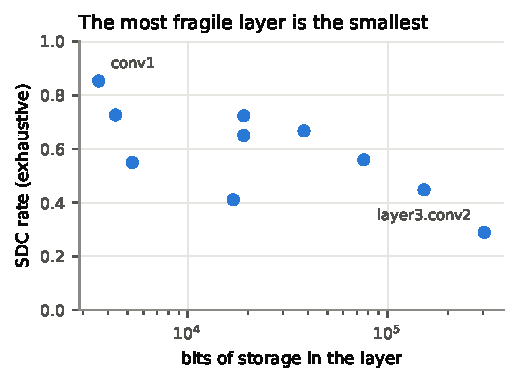
\includegraphics[width=0.52\linewidth]{fig3_layers.pdf}
\captionof{figure}{Exhaustive any-image SDC of each ResNet8 layer against its storage in bits (e4m3). The stem convolution (3{,}584 bits) is the most fragile; the last convolution (304{,}128 bits) is the most robust.}
\end{center}

\subsection{Ten seeds per width}
You retrained the whole width sweep on the GPU with ten seeds per width: 50 networks, 150 campaigns, 450{,}000 injections, all trained and measured on one device. The capacity slope $\mathrm{d}\log(\text{SDC})/\mathrm{d}\log(\text{params})$ (F29):
\begin{center}
\small
\begin{tabular}{lcc}
\toprule
format & special codes & slope \\
\midrule
e3m2 & 0 & $-1.095\pm0.098$ \\
e4m3 & 2 & $-0.705\pm0.038$ \\
e5m2 & 8 & $-0.495\pm0.032$ \\
\bottomrule
\end{tabular}
\end{center}
Paired within a seed (the same trained model for all three formats, so model-to-model variance cancels): e3m2$-$e4m3 $=-0.390\pm0.097$ ($t=-4.00$, negative in 9/10 seeds); e4m3$-$e5m2 $=-0.210\pm0.052$ ($t=-4.01$, 8/10); e3m2$-$e5m2 $=-0.600\pm0.075$ ($t=-8.01$, 10/10). \textbf{Both adjacent pairs separate, and the slopes are monotone in special-code count.}
The simple endpoint-ratio test held in only 5 of 10 seeds (F30): it throws information away. The lesson: use the statistic with the most power and say so. The control stayed clean (F31): non-finite rate e4m3 0.0107--0.0128 ($1.20\times$), e5m2 0.0714--0.0774 ($1.08\times$), e3m2 exactly 0; model-to-model spread still about $9.8\times$ the injection uncertainty.

\subsection{A vision transformer}
2.69M parameters, three seeds, 80.4--81.9\% on CIFAR-10. Quantised accuracy within 0.2 points of FP32 for every format except MXFP4 (e4m3 0.8193, e2m3 0.8190, e5m2 0.8174, e3m2 0.8173, e2m1 0.8108, FP32 0.8194). The cleanest matched-accuracy comparison of the project (F32):
\begin{center}
\small
\begin{tabular}{lcccc}
\toprule
format & NaN/Inf codes & element SDC & element non-finite & scale SDC / element SDC \\
\midrule
e5m2 & 8 & $0.0730\pm0.0089$ & 0.0689 & $3.4\times$ \\
e4m3 & 2 & $0.0453\pm0.0296$ & 0.0124 & $12.1\times$ \\
e3m2 & 0 & $0.0041\pm0.0047$ & 0.0000 & $156\times$ \\
e2m3 & 0 & 0.0236 & -- & $21.0\times$ \\
e2m1 & 0 & 0.0500 & -- & $8.6\times$ \\
\bottomrule
\end{tabular}
\end{center}
e5m2 and e3m2 differ by \textbf{0.01 points of accuracy} yet e5m2 is $17.8\times$ more vulnerable (any-image), and 94\% of its element failures are non-finite (27\% for e4m3). F18 had predicted a transformer would behave this way, and it does, more sharply, because the ViT is accurate enough that ordinary perturbations rarely flip a prediction while a NaN always does.
Neither LayerNorm nor the softmax masked the damage. Scale faults also gave non-finite outputs in 7--10\% of cases for \emph{every} format (including those without special element codes), because E8M0 has its own NaN code and its top bit is worth 128 exponent steps (F33).

One result did not fit (F34): e3m2 and e2m3 are both 6-bit, NaN-free and equally accurate, yet differ $5.8\times$ in element SDC (0.0041 against 0.0236). Special codes cannot explain that.

% =====================================================================
\section{Phase 7: The 6-bit puzzle, sensitivity and a severity measure that works (22--25 Sept)}
\markboth{Phase 7}{Phase 7}

\subsection{Ruling things out (E08--E10, F35)}
Pooled over three ViT seeds the gap is 35/8604 against 203/8604 failures (Fisher exact $p=2.5\times10^{-30}$), spread uniformly across bits and layers. You tested explanations one by one and refuted each:
\begin{itemize}
\item \textbf{Not perturbation size.} Enumerating every (element, bit) pair exactly, e2m3 perturbs weights \emph{less} than e3m2 (mean $|\Delta w|$ 0.656 against 0.717 layer-RMS units). Yet within matched perturbation bins e2m3 fails $7.0\times$ more often (0.1045 against 0.0178 in the largest bin).
\item \textbf{Not which weights are hit.} In matched bins the two strike weights of similar magnitude; renormalising per output neuron changes the gap not at all ($6.4\times$ against $6.3\times$).
\item \textbf{Not margin compression.} Median normalised margins 2.853 against 2.863.
\end{itemize}

\subsection{The fragility belongs to the quantised network (F36)}
You perturbed one random weight by a fixed multiple of the layer RMS, a probe with no bit patterns in it at all:
\begin{center}
\small
\begin{tabular}{lcccc}
\toprule
network & mantissa bits & $0.5$ rms & $1.5$ rms & $3.0$ rms \\
\midrule
e5m2 & 2 & 0.0000 & 0.0000 & 0.0013 \\
e3m2 & 2 & 0.0000 & 0.0000 & 0.0013 \\
e4m3 & 3 & 0.0080 & 0.0493 & 0.1380 \\
e2m3 & 3 & 0.0013 & 0.0187 & 0.0513 \\
e2m1 & 1 & 0.0160 & 0.0740 & 0.1407 \\
\bottomrule
\end{tabular}
\end{center}
At 1.5 RMS the 2-mantissa networks never flipped a prediction in 1{,}500 trials; the 3-mantissa networks flipped 2--5\% of the time. Since the probe never touches a code, the difference cannot come from how faults are encoded: \emph{two quantised networks of equal accuracy and margins can differ by more than an order of magnitude in how a weight perturbation of a given size disturbs them.}
You first wrote this as ``mantissa width tracks vulnerability'' (F37).

\subsection{A sensitivity measure (E11, F38)}
Let $m=z_{(1)}-z_{(2)}$ be an image's margin. Moving weight $w_i$ by $\delta$ shifts the margin by about $\delta\,\partial m/\partial w_i$ to first order, and the prediction flips when this exceeds $m$. So define the dimensionless \emph{sensitivity}
\[
s_i=\frac{|\partial m/\partial w_i|\cdot\mathrm{rms}}{m},
\]
maximised over the evaluation images (a weight fault is exposed to all of them), where rms is the layer's weight RMS. A perturbation of $\delta\cdot\mathrm{rms}$ should flip a prediction roughly when $s_i\delta>1$. $s$ is computed by backpropagation, one pass per image. It predicts the format-agnostic probe at \textbf{correlation $+0.998$} across 15 (format, size) cells. For example at 1.5 rms, predicted against measured: e4m3 0.0471/0.0493; e2m3 0.0154/0.0187; e2m1 0.0677/0.0740.
Decomposing $s$: mean margin (3.59 against 3.63), logit spread and mean $|\partial m/\partial w|\cdot$rms agree across formats to three digits; only the \emph{tail} differs (99th percentile 0.161 against 2.309).

\subsection{Extending to all five formats breaks the mantissa story (F45)}
\begin{center}
\small
\begin{tabular}{lcccc}
\toprule
format & mantissa & accuracy & median $s$ & perturbation-driven SDC \\
\midrule
e5m2 & 2 & 0.8174 & 0.0122 & 0.0040 \\
e3m2 & 2 & 0.8173 & 0.0121 & 0.0041 \\
e4m3 & 3 & 0.8193 & 0.1249 & 0.0329 \\
e2m3 & 3 & 0.8190 & 0.0492 & 0.0236 \\
e2m1 & \textbf{1} & 0.8108 & \textbf{0.1187} & \textbf{0.0500} \\
\bottomrule
\end{tabular}
\end{center}
e2m1 has the \emph{fewest} mantissa bits and the \emph{highest} perturbation failure rate. Across the five formats, median sensitivity predicts perturbation-driven SDC at $r=+0.925$; mantissa bits at $r=-0.251$. Mantissa width was a correlate inside one group of formats, not a cause. The design guidance changed from ``prefer coarser mantissas'' (unsupportable) to: avoid special codes, and \emph{measure $s$ on the quantised network}.

\subsection{A severity measure that predicts failure (E12, F39)}
For a fault changing a weight from $v$ to $v'$:
\[
\mathrm{margin\_shift}_i=s_i\cdot\frac{|v_i'-v_i|}{\mathrm{rms}},
\]
the fraction of the decision margin the fault uses up. Four measures were compared over 39{,}337 ViT element faults that stayed finite:
\begin{center}
\small
\begin{tabular}{lccp{5.4cm}}
\toprule
measure & AUC & Spearman & what it knows \\
\midrule
\code{log_severity} (the proposal's $d$) & \textbf{0.435} & $-0.035$ & number system only \\
\code{rel_error} $=|v'-v|/|v|$ & 0.699 & 0.107 & number system only \\
\code{delta_rms} $=|v'-v|/\mathrm{rms}$ & 0.845 & 0.184 & number system and layer scale \\
\code{margin_shift} & \textbf{0.990} & 0.261 & number system and the network \\
\bottomrule
\end{tabular}
\end{center}
The proposal's measure ranks failures slightly worse than chance. Its threshold needs no tuning: flagging $\mathrm{margin\_shift}>1$ catches \textbf{98.5\%} of all failures while flagging \textbf{4.4\%} of the fault space (precision 0.544).
\begin{center}
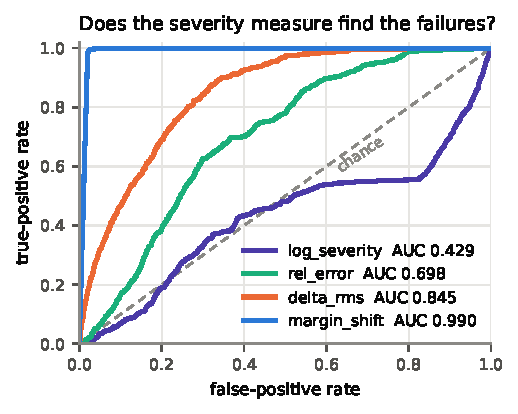
\includegraphics[width=0.55\linewidth]{fig4_severity.pdf}
\captionof{figure}{ROC curves: how well each severity measure ranks the faults that actually failed. A curve on the diagonal is chance; the proposal's \code{log_severity} sits below it, \code{margin_shift} hugs the top-left corner.}
\end{center}
(The figure legend shows AUC 0.429 and 0.698 for the first two measures while the report text says 0.435 and 0.699; they are computed on slightly different fault subsets. See the list of items to double-check in Section~\ref{app:check}.)
It also carries a caveat: severity is \emph{not} a property of the number system alone, since the same flip in the same format has different consequences in two networks of equal accuracy.

\subsection{Firming up, and a first test of value-aware sampling}
\begin{itemize}
\item \textbf{Second exhaustive campaign} (F41): e3m2, 483{,}904 injections, in which \emph{not one fault} produced a non-finite value; the sample again covered the truth (0.1070 [0.0964, 0.1186] against truth 0.1079). Scale/element $10.2\times$.
\item \textbf{RepVGG with three seeds} (F42; 91.45\% each): e5m2 element 0.0583 (non-finite 0.0538, i.e.\ 92\%), e4m3 0.0107, e3m2 0.0012 (non-finite 0). Scale/element $5.1\times$, $28.7\times$, $232\times$.
\item \textbf{Value-aware sampling against exhaustive ground truth} (E15, F46--F47; replayed 400 times without new injections). Splitting the fault space at $\mathrm{margin\_shift}$ of 0.1 and 1.0: on e3m2 the low stratum (38.6\% of the space) held \emph{zero} failures, the high stratum (14.2\%) had rate 0.744. Neyman allocation with a 20\% pilot gave a \textbf{$7.0\times$ variance reduction} on e3m2 (AUC 0.989) and $2.1$--$2.3\times$ on e4m3 (AUC 0.882),
 growing as the failure rate falls. (The first version reported no gain on e4m3 because of the checkpoint mismatch in Phase 8.)
\end{itemize}

\subsection{What $s$ really measures: the last open question (E16, E17; F48, F49)}
You had concluded by elimination that the difference in $s$ between formats must be \emph{alignment} (whether per-position terms of the gradient reinforce each other). Elimination is only as good as the list. A permutation test destroyed the alignment while preserving every value of both marginals: the tail moved by at most 2\% (gain $1.00$--$1.02\times$ for all formats), so the guess was wrong.
Splitting $s$ into its two factors gave the answer:
\begin{center}
\small
\begin{tabular}{lc}
\toprule
quantity & spread across the five formats \\
\midrule
$s$, median & $10.29\times$ \\
$s$, 99th percentile & $22.24\times$ \\
gradient factor $|\partial m/\partial w|\cdot\mathrm{rms}$ & $\approx1.01$--$1.08\times$ \\
$s$ with the margin divided out (median and 99th percentile) & \textbf{$1.08\times$} \\
\bottomrule
\end{tabular}
\end{center}
The gradient field is the same in every format. The entire spread comes from the margin of \emph{one} evaluation image, the closest to a decision boundary (smallest margin 0.0070 for e2m1 against 0.2330 for e5m2, a $33\times$ range), and because $s$ is defined as a maximum over images, that one image raises $s$ for every weight at once.
And that image belongs to the evaluation set rather than the network: $1/\min m$ ranked fifteen networks (3 seeds $\times$ 5 formats) by failure rate at Spearman $+0.983$ on the campaign's own 200 images but only $+0.209$ on 2{,}000 fresh images. The seed-to-seed component of vulnerability is a real property of the network (Spearman $+1.000$ on fresh images in all 5 formats),
but the format-to-format component, at 200 images, is a property of the (network, evaluation set) pair.

% =====================================================================
\section{Phase 8: Two mistakes caught, and the change of metric (25--27 Sept)}
\label{sec:phase-metric}
\markboth{Phase 8}{Phase 8}

\subsection{Mistake one: the campaigns were recorded on different networks (F50)}
Training is not bit-reproducible across machines. Of the 24 checkpoint names existing on both the laptop and the cluster, \textbf{none} has identical weights, yet accuracies agree within a few tenths of a point. You wrote a replay check: take 300 recorded faults, re-inject them in the checkpoint in hand, compare outcomes.
\begin{center}
\small
\begin{tabular}{lcc}
\toprule
exhaustive campaign & agrees with checkpoint A & agrees with checkpoint B \\
\midrule
e3m2, 483{,}904 faults & 253/300 & \textbf{300/300} \\
e4m3, 638{,}624 faults & \textbf{300/300} & 202/300 \\
\bottomrule
\end{tabular}
\end{center}
The two exhaustive campaigns were recorded on \emph{two different trained networks}. So the comparison you had quoted as ``exhaustive confirmation'' of the mantissa effect (element rates 0.0785 for e3m2 against 0.4003 for e4m3, a factor of five) put one network's e3m2 next to another network's e4m3, and given the tenfold network-to-network spread it said nothing about the formats.
The first version of the e4m3 sampling result (AUC 0.705, ``no gain'') had the same flaw; matched, it is AUC 0.882 and $2.3\times$. Since then every campaign is tied to its checkpoint, the replay check runs automatically, and the two exhaustive campaigns are used as two independent references, never as a format comparison.

\subsection{Mistake two: the metric itself (F51, F52)}
To redo the comparison properly you replayed one fixed list of 1{,}500 element faults per format against \textbf{nine disjoint, class-balanced sets of 200 images}, on each of two networks. (On network A's original images the e4m3 rate came out 0.4087 against its exhaustive 0.4003, so the set-up reproduces the reference.)
\begin{center}
\small
\begin{tabular}{llccc}
\toprule
metric & network & e3m2 & e4m3 & e4m3/e3m2 (per-fold range) \\
\midrule
any-image & A & 0.2152 & 0.2214 & $1.03\times$ ($0.34$--$2.58\times$) \\
any-image & B & 0.1623 & 0.1504 & $0.93\times$ ($0.47$--$2.14\times$) \\
per-inference & A & 0.00202 & 0.01124 & $\mathbf{5.57\times}$ \\
per-inference & B & 0.00129 & 0.00987 & $\mathbf{7.64\times}$ \\
\bottomrule
\end{tabular}
\end{center}
Under the any-image metric the formats look equal, their order reverses from one image set to the next, and the rate moves up to 3.8--11$\times$ its own confidence-interval width between sets, tracking each set's smallest margin (Spearman $+0.80$ to $+0.93$).
Per inference, the same faults on the same image sets give $5.6\times$ and $7.6\times$ between the formats, with the e4m3 rate stable to $1.27\times$ and $1.15\times$ across image sets. Two independently trained networks agree.

\begin{keyidea}
The any-image metric \textbf{saturates}: it grows with the number of images and tends to 1, so beyond a few dozen images it mostly reports whether the set contains a near-tie input. The Wilson interval is not wrong; it answers a narrower question than it appears to. It covers the uncertainty from sampling \emph{faults}, while the choice of evaluation images is a second and larger source that no number of injections reduces.
From here on, the \textbf{per-inference rate is the primary metric}.
\end{keyidea}

\subsection{Rescoring everything (E19, F55--F59)}
Because every campaign had always recorded \code{changed} per fault, all \textbf{119 weight campaigns (1{,}441{,}528 faults, 8 model configurations)} could be rescored per inference without a single new injection.
\begin{center}
\small
\begin{tabular}{lcccccc}
\toprule
network & seeds & e3m2 & e4m3 & e5m2 & any-image order & per-inference order \\
\midrule
RepVGG-A0 & 3 & 0.00001 & 0.00688 & 0.05381 & holds & holds \\
ViT & 3 & 0.00003 & 0.01258 & 0.06897 & holds & holds \\
ResNet8 (reference) & 1 & 0.00332 & 0.01699 & 0.07801 & reversed & holds \\
ResNet8 w8 & 5 & 0.01003 & 0.02005 & 0.08143 & reversed & holds \\
ResNet8 w16 & 5 & 0.00180 & 0.01374 & 0.07831 & holds & holds \\
ResNet8 w24 & 4 & 0.00121 & 0.01210 & 0.07585 & reversed & holds \\
ResNet8 w32 & 4 & 0.00060 & 0.01354 & 0.07934 & reversed & holds \\
ResNet8 w48 & 4 & 0.00035 & 0.01302 & 0.07812 & reversed & holds \\
\bottomrule
\end{tabular}
\end{center}
e3m2 $<$ e4m3 $<$ e5m2 holds on \textbf{8 of 8} models per inference, with disjoint 95\% intervals everywhere, against 3 of 8 under the any-image rate. So the Phase 4 finding ``the ranking reverses across architectures'' was a metric artefact. On the ViT one e5m2 element fault is about $2000\times$ as likely as one in e3m2 to corrupt a given inference, at 0.01 points of accuracy difference.

\textbf{Scale dominance survives and grows where the element rate is low} (F56): scale/element per inference: RepVGG e3m2 8424$\times$ (lower bound of order $10^3$, since the denominator is $0.00001$ [0.00000, 0.00003]); ViT e3m2 3212$\times$; ResNet8-w48 e3m2 $434\times$; ResNet8-w16 e4m3 $13.3\times$; ResNet8-w16 e5m2 $2.6\times$. The direction never reverses.

\textbf{The capacity result sharpened} (F58). Ratio of the widest to the narrowest ResNet8 ($35\times$ parameters); below 1 means capacity helps:
\begin{center}
\small
\begin{tabular}{lccc}
\toprule
format & special codes & any-image & per inference \\
\midrule
e3m2 & 0 & $0.11\times$ & \textbf{$0.04\times$} (25$\times$ better) \\
e4m3 & 2 & $0.13\times$ & $0.65\times$ \\
e5m2 & 8 & $0.27\times$ & \textbf{$0.96\times$} (no benefit) \\
\bottomrule
\end{tabular}
\end{center}
96.9\% of e5m2's per-inference element damage is non-finite. Capacity absorbs perturbations and cannot absorb a NaN.
\begin{center}
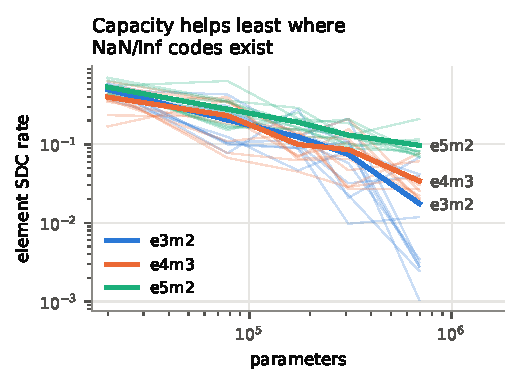
\includegraphics[width=0.58\linewidth]{fig2_capacity.pdf}
\captionof{figure}{Per-inference rate of element faults against parameter count, ResNet8 at five widths. Faint lines are single trained networks, bold lines are means. Capacity helps most where there are no special codes, and not at all for e5m2.}
\end{center}

\textbf{Block-size story weaker than first claimed} (F57): per inference, a genuine monotone block-size trend exists under both scale rules (RepVGG e4m3: OCP spread $5.76\times$, fit $4.66\times$; ResNet8: $1.77\times$ and $1.43\times$). \textbf{The sensitivity result needed no change} (F59): correlations of median $s$ with perturbation-driven SDC were identical to three decimals under both metrics ($+0.928$ against mantissa bits $-0.248$ and $-0.225$).

\subsection{Value-aware sampling, re-derived for the per-inference rate (E20, F60, F61)}
The earlier gains were for the any-image rate, so they were redone. The target changes shape: on ResNet8 under e3m2, \textbf{89.2\%} of the 483{,}904 faults corrupt \emph{no} inference at all; among the other 10.8\% the mean corruption is 0.081 (about 16 images) and the maximum is 1.0.
The estimator changes too. A per-inference rate is a \emph{mean of per-fault proportions}, so each stratum's variance has to be estimated from the pilot instead of assumed to be $p(1-p)$, and Neyman allocation becomes $n_k\propto w_k\sigma_k$.
\begin{center}
\small
\begin{tabular}{p{6.6cm}cc}
\toprule
stratification & e3m2 variance ratio & e4m3 variance ratio \\
\midrule
fixed cuts (0.1 and 1, tuned for the old target) & $6.8$--$8.3\times$ & $1.5$--$1.8\times$ \\
quantile cuts of the score (50/75/90/97/99.5th percentiles, 6 strata); budgets 500/1000/3000 & $120/102/115\times$ & $64/83/57\times$ \\
equivalent uniform budget at 3{,}000 & 346{,}106 & 171{,}165 \\
\bottomrule
\end{tabular}
\end{center}
Both estimators are unbiased at every budget. Why quantile cuts: the rank correlation of the score with the per-inference rate is only moderate ($\rho=0.53$ to $0.70$), but the job is not to rank everything well, it is to \emph{isolate the thin high-value tail}, and the data's own top percentiles do that. A 3{,}000-injection stratified campaign matches a uniform campaign of 171{,}000 to 346{,}000.
This supersedes the earlier any-image figures as sampling guidance.

% =====================================================================
\section{Phase 9: The proposal's two open design choices (28 Sept--1 Oct)}
\markboth{Phase 9}{Phase 9}

\subsection{Single-bit or multi-bit? (E21, F62--F64)}
\label{sec:multibit}
The proposal adopted single-bit flips and listed the multi-bit H-model as an open extension. Design: on each of two ResNet8-w16 networks and in each of e3m2, e4m3, e5m2, sample 1{,}500 element words and 500 scale bytes and inject \emph{every} single-bit and \emph{every} two-bit pattern of each word: \textbf{390{,}000 injections}, recording which images changed.
(Check: the single-bit rates reproduce the exhaustive campaign: e3m2 element 0.00103 against 0.00113, scale 0.1875 against 0.1887.)
\begin{center}
\small
\begin{tabular}{llcc}
\toprule
format & site & $r_2/r_1$ (random double / single), two networks & adjacent$/r_1$ \\
\midrule
e3m2 & element & 1.55 / 1.42 & 0.94 / 0.93 \\
e4m3 & element & 1.11 / 1.20 & 1.10 / 1.13 \\
e5m2 & element & 1.04 / 1.04 & 0.86 / 0.88 \\
e3m2 & scale & 1.48 / 1.46 & 1.06 / 1.05 \\
e4m3 & scale & 1.32 / 1.30 & 0.85 / 0.85 \\
e5m2 & scale & 1.46 / 1.45 & 1.01 / 1.01 \\
\bottomrule
\end{tabular}
\end{center}
A double flip corrupts $1.04$--$1.55\times$ as many inferences as a single flip, and an \emph{adjacent} double (the pattern a multi-cell upset produces) $0.85$--$1.13\times$. The format ordering and scale dominance are unchanged. Double flips are \textbf{sub-additive}, doing only 52--85\% of the union of their two single flips, for two reasons:
\begin{itemize}
\item a second flip can move a word \emph{off} the NaN code its partner would have reached (a special code is one bit pattern, and flipping another bit leaves it);
\item two scale bits of opposite value cancel: $X\oplus(2^a+2^b)$ shifts $X$ by $\pm(2^b-2^a)$; for adjacent scale bits 2 and 3 on e3m2, 0.21 and 0.19 singly but 0.08 together.
\end{itemize}
Plugging the measured rates into the H-model's own expansion, with per-bit probability $p$ and word width $W$,
\[
\text{expected damage}=\sum_b p(1-p)^{W-1}r_b+\sum_{a<b}p^2(1-p)^{W-2}r_{ab}+O(p^3),
\]
the double-flip term reaches 1\% of the total only at $p=1.9$--$2.9\times10^{-3}$, and 10\% at $p\approx2$--$3\times10^{-2}$. At $p=2\times10^{-3}$ ResNet8-w16's 484k--639k weight bits already contain about 1{,}000--1{,}300 flipped bits at once, so the one-fault-per-inference assumption fails through \emph{accumulation across words}
three orders of magnitude in $p$ before multiplicity \emph{within} a word matters. \textbf{Settled: single-bit injection is sufficient.}

\subsection{Learned intervals or exact enumeration? (E22, F65, F66)}
The second open choice, inherited from TreeFI. Every strategy is replayed against the two exhaustive campaigns 400 times per budget and scored by the variance of its per-inference estimate relative to uniform sampling (both networks replay-verified, 200/200). Variance ratio over uniform at budgets 500/1000/3000 with 6 strata:
\begin{center}
\small
\begin{tabular}{lcc}
\toprule
arm & e3m2 & e4m3 \\
\midrule
learned tree (value) & $0.33/0.36/0.98$ & $0.18/0.14/0.25$ \\
learned tree (value + layer) & $0.10/0.11/0.69$ & $0.13/0.13/0.20$ \\
\ldots with proportional allocation & $0.80/0.90/0.84$ & $0.82/0.97/0.86$ \\
\textbf{exact $|\Delta v|/\mathrm{rms}$ enumeration} & $\mathbf{48/48/55}$ & $\mathbf{65/65/60}$ \\
exact \code{margin_shift} (adds the gradient) & $99/127/114$ & $74/83/74$ \\
\bottomrule
\end{tabular}
\end{center}
The learned tree never beats uniform sampling. Exact enumeration of the decoded change alone (table look-ups and one RMS per layer, no gradient, no injections) cuts variance $48$--$65\times$; adding the gradient roughly doubles it on e3m2 but adds only 15--30\% on e4m3, so most of the gain comes from enumerating the code table exactly.
Why learning fails (F66):
\begin{itemize}
\item \textbf{A pilot cannot see a zero-inflated tail.} With 89\% of faults corrupting nothing, a pilot of 100--600 faults sees a handful of failures; leaves where none were seen get zero variance, Neyman starves them, and they hold variance after all. (A tree fitted to the \emph{whole} truth, an oracle, reaches $20$--$39\times$ at 6 leaves, so the information is in the features; learning it is what costs more injections than it saves.)
\item \textbf{On e4m3 the tail is a set of discrete codes.} $1.27\%$ of e4m3's element faults (7{,}853 of 618{,}880) are (code, bit) pairs that flip into NaN; each corrupts every inference ($r=1.000$), together carrying 77.6\% of element damage and 52.2\% of all damage in the model. They are properties of specific bit patterns, not of a value range, so a partition of value space spreads them thinly. A code table identifies all of them exactly.
\end{itemize}
\textbf{Settled:} for MX, characterise impact by exact per-code enumeration. TreeFI's interval learning solves a problem (an alphabet of $2^{32}$ values) that MX does not have.

\subsection{The sign bit, revisited (F67)}
\begin{center}
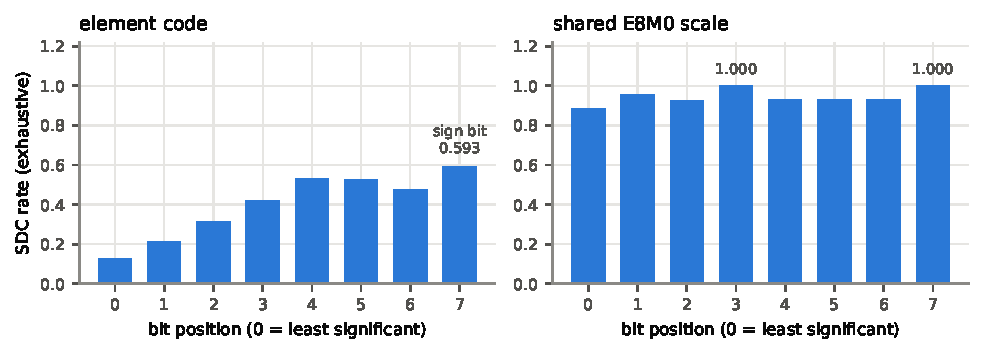
\includegraphics[width=\linewidth]{fig1_per_bit.pdf}
\captionof{figure}{Exhaustive damage per bit, per inference (ResNet8-w16, e4m3, $K=32$, 638{,}624 injections), split by whether the output stayed finite. Left: element bits. Right: scale bits.}
\end{center}
Among faults whose output stays finite, the sign bit is still the worst element bit ($0.0073$ against $0.0052$ for the next). But in total damage it ranks \textbf{seventh of eight} in e4m3: the 1.27\% of element faults that flip into the NaN code each corrupt every inference and carry 77.6\% of all element damage, with 85--95\% of the damage of every bit from 0 to 4 being non-finite.
A sign flip never changes the magnitude bits, so it is the one bit that can never reach NaN. The any-image metric hid this because a sign flip changes \emph{some} image in 59\% of cases but few of them, while a NaN flip changes all 200 and scores the same single unit.

On the scale (bytes lie in 114--120 on this network, so bits 4--6 are always set and bit 3 almost never): flipping bit 3 multiplies the block by 256 and corrupts 75\% of inferences, bit 7 overflows it (98\%), while flipping bits 4--6 divides the block towards zero and corrupts only 3\%. \textbf{Growing a block is catastrophic; shrinking it is mild.}

% =====================================================================
\section{Phase 10: A read-side guard for special codes (1--2 Oct)}
\markboth{Phase 10}{Phase 10}
If most element damage comes from one transition, into a special code, an obvious defence is to \textbf{decode any special element code as zero when it is read}. A fault that would have produced NaN then merely zeroes one weight.

\textbf{Method (E23).} Every element fault that lands on a special code is found by enumeration, so its share $f$ of the element space is exact. 1{,}000 of them are injected twice (unguarded and guarded); 2{,}000 uniformly drawn \emph{other} element faults are injected once (the guard does not change them). Then
\[
\text{rate}_{\text{unguarded}}=f\,\bar r_{\text{special}}+(1-f)\,\bar r_{\text{other}},\qquad
\text{rate}_{\text{guarded}}=f\,\bar r_{\text{special, guarded}}+(1-f)\,\bar r_{\text{other}},
\]
needing no earlier campaign and so unable to be scored against the wrong network. Check: against ResNet8 train-seed 9's exhaustive e4m3 campaign the sampled estimate is $0.016357\to0.003749$ against exhaustive $0.016354\to0.003747$, four significant digits.

\begin{center}
\small
\begin{tabular}{@{}llp{2.9cm}p{2.9cm}p{2.6cm}@{}}
\toprule
network & format & special faults, share of space & share of element damage & reduction, at least \\
\midrule
ResNet8 (2 nets) & e4m3 & 1.27--1.29\% & 77.6--92.8\% & $3.9$--$10.7\times$ \\
ResNet8 (2 nets) & e5m2 & 7.6--7.7\% & 97.5--98.7\% & $30$--$53\times$ \\
RepVGG-A0 (3 seeds) & e4m3 & 0.80\% & 99.5--99.9\% & $115$--$389\times$ \\
RepVGG-A0 (3 seeds) & e5m2 & 5.35--5.38\% & 99.9--100\% & $319$--$4112\times$ \\
ViT (3 seeds) & e4m3 & 1.12--1.13\% & 97.1--99.5\% & $29$--$133\times$ \\
ViT (3 seeds) & e5m2 & 6.86--6.95\% & 99.9--100\% & $43$--$2479\times$ \\
\bottomrule
\end{tabular}
\end{center}
The reduction is the unguarded rate divided by a 95\% \emph{upper bound} on the guarded rate, so it is a lower bound. Unguarded, a special-code fault corrupts 99.95--100\% of inferences; guarded, essentially none, on all sixteen networks and formats, and no guarded fault produced a non-finite output.
Guarded e5m2 lands in the same range as e3m2's element rate on RepVGG and the ViT. On ResNet8 the reduction is smaller because a small network is also fragile to ordinary perturbations, which the guard does not touch. A guarded special code still costs one weight (it reads as zero), which is why the guarded rate is not exactly zero.
The guard was \emph{simulated in software}; in hardware it is one comparator on the read path. It turns ``prefer formats without special codes'' from a constraint into a choice.

% =====================================================================
\section{Phase 11: A bug in your own codec, and a harder dataset (2--3 Oct)}
\label{sec:phase-c100}
\markboth{Phase 11}{Phase 11}

\subsection{The codec bug (F69)}
While preparing activation experiments for CIFAR-100 you noticed that \emph{no activation campaign, on any model, had ever recorded a non-finite output}, although enumeration showed that activations have the same share of special-code faults as weights (1.1--1.4\% across ten images against 1.24\%). The cause: \code{quantize()} mapped a NaN input to zero. An activation-quantised layer re-encodes its input,
so a NaN created by an activation fault was erased by the next layer. The OCP conversion does the opposite: the shared scale is taken from the block maximum, so a NaN anywhere in a block makes the whole block NaN (Algorithm~1 of the MX paper). You fixed the codec, added a test that pins the behaviour, and reran every activation campaign (100 images, 4{,}000 faults), each on the checkpoint that produced the weight campaign it is compared with.
Weight campaigns were unaffected, since trained weights contain no NaN to re-encode. The old outputs are kept in \code{cluster/archive/e04_buggy_codec/}.

\begin{center}
\small
\begin{tabular}{llccc}
\toprule
network & format & weight & activation [95\% CI] & weight/activation \\
\midrule
ResNet8 & e4m3 & 0.0170 & 0.0122 [0.0077, 0.0182] & $1.4\times$ \\
RepVGG-A0 & e4m3 & 0.0048 & 0.0075 [0.0049, 0.0101] & $0.64\times$ \\
ViT & e4m3 & 0.0122 & 0.0114 [0.0080, 0.0150] & $1.07\times$ \\
ResNet8 & e5m2 & 0.0780 & 0.0359 [0.0302, 0.0421] & $2.2\times$ \\
RepVGG-A0 & e5m2 & 0.0549 & 0.0378 [0.0319, 0.0442] & $1.45\times$ \\
ViT & e5m2 & 0.0659 & 0.0486 [0.0420, 0.0554] & $1.36\times$ \\
\bottomrule
\end{tabular}
\end{center}
The corrected numbers \textbf{withdraw} the earlier claim that activation faults barely matter on the larger models (it had said, for example, that none of 2{,}000 transformer activation faults changed an inference). Per inference an element fault in a weight does $0.3$--$2.2\times$ the damage of one in an activation, and under e4m3 the two are statistically indistinguishable on CIFAR-10.
Same reason in both tensors: about 1\% of faults land on a special code and destroy the inference. The real difference is \emph{exposure}: a weight fault persists across every inference until the memory is rewritten; an activation fault lives for one. Scale faults dominate in both ($14\times$ in activations and $11\times$ in weights on ResNet8).
(The lesson you drew: an absent non-finite output where one was expected is what exposed the bug.)

\subsection{CIFAR-100 in place of ImageNet (E24, F70--F72)}
The proposal's transformer study was DeiT on ImageNet, which no machine you could use held. CIFAR-100 was the nearest affordable substitute: ten times the classes and a tenth of the images per class, so networks sit much closer to decision boundaries, which is exactly the property the margin results had shown to matter. All three architectures were retrained with unchanged recipes, three seeds each:
ResNet8 58\%, RepVGG-A0 70--71\%, ViT 47--49\%. Every campaign scores 200 images (2 per class).

\textbf{Everything replicated} (F70): formats matched in accuracy (four formats within 0.01 points on the ViT); e3m2 $<$ e4m3 $<$ e5m2 on all nine networks; scale faults outweigh element faults everywhere ($1.7\times$ to $3600\times$); NaN codes carry 94--100\% of e4m3/e5m2 element damage on the larger models.

\textbf{What changed was the floor} (F71):
\begin{center}
\small
\begin{tabular}{lcccc}
\toprule
network & e3m2 (no special codes) & e4m3 & e5m2 & e4m3/e3m2 gap \\
\midrule
ViT & $2.7\text{e-}5\to6.1\text{e-}4$ ($22\times$) & $0.0126\to0.0114$ & $0.069\to0.077$ & $461\times\to19\times$ \\
RepVGG-A0 & $1.4\text{e-}5\to5.6\text{e-}5$ ($3.9\times$) & $0.0069\to0.0081$ & $0.054\to0.057$ & $476\times\to144\times$ \\
ResNet8 & $1.8\text{e-}3\to5.7\text{e-}3$ ($3.2\times$) & $0.0137\to0.0169$ & $0.078\to0.082$ & $7.6\times\to3.0\times$ \\
\bottomrule
\end{tabular}
\end{center}
With smaller margins the formats without special codes became $3$--$22\times$ more vulnerable, while e4m3 and e5m2 barely moved, since a NaN corrupts an inference however wide the margins are. So the gap narrows: the advantage of NaN-free formats is smaller exactly on the harder tasks real deployments face. Among NaN-free formats the ordering does \emph{not} carry over:
on CIFAR-10 the ViT ranks e3m2 $<$ e2m3 $<$ e2m1, on CIFAR-100 e2m1 $<$ e2m3 $\approx$ e3m2, on all three seeds, which is what the sensitivity result predicts. The read-side guard still works, with reductions of at least $13$--$1387\times$ on RepVGG and $24$--$168\times$ on the ViT (ResNet8: $3.5$--$16\times$) (F72).

% =====================================================================
\section{Phase 12: Wrap-up (3--5 Oct)}
\markboth{Phase 12}{Phase 12}
The last runs added seeds to ResNet8 on CIFAR-100 and repeated the activation campaigns under e5m2 on all six models (weight/activation $0.3$--$2.2\times$; e5m2 weights $1.4$--$2.2\times$ worse on CIFAR-10 because fewer activation faults reach a special code). On 3 October you pushed the library, every experiment script, the trained networks and the raw campaign outputs to the repository.
On 5 October the report was rewritten as a 13-page document organised around the five objectives, with sections on methodological findings, design guidance and limitations, and the ImageNet gap stated openly.

\textbf{Totals.} About 1.44 million sampled weight faults in 119 campaigns on CIFAR-10; two exhaustive campaigns (1.12 million injections); 390{,}000 multi-bit injections; further campaigns for activations, the NaN guard and CIFAR-100; more than sixty independently trained networks; 72 numbered findings including those later revised.

\part{The results as a whole}

\section{The five objectives, answered}
\markboth{Objectives answered}{Objectives answered}
All rates are per inference unless stated.

\begin{center}
\small
\begin{longtable}{@{}p{2.5cm}p{12.9cm}@{}}
\toprule
\textbf{O1} Fault propagation & A scale fault is always more damaging than an element fault, typically $13\times$ to over $1000\times$, on every architecture, format, tensor type and dataset. The exception is e5m2 ($2.6\times$), whose element faults are already NaN-dominated. Scale faults also give non-finite outputs in 7--13\% of cases for every format, because E8M0 has its own NaN code and its top bit is worth 128 exponent steps.
 Exhaustive numbers (ResNet8-w16, e4m3): scale 0.9442 against element 0.4003 any-image; 49.9 against 3.27 images changed. \\
\textbf{O2} Format sensitivity & Formats of equal accuracy differ by up to three orders of magnitude. e3m2 $<$ e4m3 $<$ e5m2 on all eight CIFAR-10 configurations and all nine CIFAR-100 networks, with disjoint intervals. On the ViT a single e5m2 element fault is about $2000\times$ as likely as an e3m2 one to corrupt an inference, at 0.01 points of accuracy difference. \\
\textbf{O3} Block size & Larger blocks shrink the scale's share of storage ($11.1\%\to1.7\%$) but make each scale fault worse ($40.1\to50.1$ images changed), while element faults become milder (per-inference $0.0241\to0.0136$). A genuine trade-off; with protected scales, large blocks are safe. OCP clipping exaggerates the any-image trend but does not create it. \\
\textbf{O4} Tensor and location & Per fault, weights and activations are about equally dangerous ($0.3$--$2.2\times$): about 1\% of faults in either land on a special code. They differ in \emph{exposure}: weight faults persist, activation faults last one inference. Among finite faults the sign bit is the worst element bit, but flips into NaN dominate total damage. In the scale, flips that grow a block are catastrophic and flips that shrink it are mild. The small stem layer is the most fragile layer (0.853 against 0.289 for the largest). \\
\textbf{O5} Vulnerability drivers & (1) The NaN/Inf codes: they carry 97--100\% of element damage on the larger models, capacity cannot absorb them, and a read-side guard removes them. (2) For the remaining perturbation damage: the network's margin-normalised sensitivity ($r=+0.93$ across formats), not mantissa or exponent width, with the per-set margins of the hardest evaluation image mattering for any-image metrics. \\
\bottomrule
\end{longtable}
\end{center}

\begin{center}
\small
\begin{longtable}{@{}p{5.2cm}p{10.1cm}@{}}
\toprule
\textbf{Expected outcome in the proposal} & \textbf{What was found} \\
\midrule
\endhead
Shared-scale faults have a significantly different, typically larger, impact & Confirmed everywhere; never reversed. \\
Reliability varies across formats at comparable accuracy & Confirmed by up to three orders of magnitude; explained by special codes and network sensitivity. \\
A block-size trade-off & Confirmed, with the two fault sites moving in opposite directions. \\
Per-tensor and per-location sensitivity maps & Exhaustive per-bit and per-layer maps for ResNet8; weight/activation comparison on six models. \\
Design guidance & Section~\ref{sec:guidance}, including a read-side guard the proposal did not anticipate. \\
Open choice: learned versus exact intervals & Settled: exact enumeration, $48$--$65\times$ against $\le1\times$ (with the caveat about what ``learned'' meant, Part~II). \\
Open choice: single versus multi-bit & Settled: single-bit is sufficient. \\
Open choice: the grid actually swept & All five formats and four block sizes on CIFAR; DeiT/ImageNet replaced by a ViT on CIFAR-100. \\
\bottomrule
\end{longtable}
\end{center}

\section{The two mechanisms behind vulnerability, in plain words}
\markboth{Two mechanisms}{Two mechanisms}

\subsection{Mechanism 1: the NaN pathway}
\begin{enumerate}
\item In e4m3 and e5m2 a small fraction of element faults (about 1\% in e4m3, about 5--8\% in e5m2) flip a code into NaN or Infinity.
\item That value propagates: every output of the layer is NaN, then every later output, so \emph{every inference} is wrong.
\item Whether the format has such codes is a property of the \emph{format}. Whether a flip lands on one depends on the stored value (codes one flip away from \ee{S.1111.111}), not on the network. So the non-finite rate does not change with model width (e5m2 varied by $1.08\times$ across a $35\times$ capacity range).
\item Ordinary perturbations \emph{do} get absorbed as the network gets bigger and more accurate. So as capacity grows, the NaN share of the damage grows (e5m2: 16\% to 66\% of failures in the first sweep; 97\% on the larger networks).
\item Formats without special codes cannot suffer this. A read-side guard that decodes special codes as zero removes it.
\end{enumerate}
The size of this effect is why formats of equal accuracy differ by up to three orders of magnitude.

\subsection{Mechanism 2: sensitivity and margins (for everything that is not NaN)}
Perturbation damage depends on how close the network's decisions are to a tie. The sensitivity $s_i=|\partial m/\partial w_i|\,\mathrm{rms}/m$ measures the fraction of the margin $m$ that one weight can move, and predicts the failure rate of a fixed-size perturbation at $+0.998$.
Two further facts: (i) between formats the gradient factor of $s$ is the same ($1.08\times$) and the whole spread comes from the margin of the \emph{closest-to-a-tie} image among the evaluation images; (ii) lower margins (harder tasks) raise perturbation damage but leave the NaN pathway untouched, which is why the format gap narrows on CIFAR-100.

\subsection{How the mechanisms combine}
\begin{center}
\small
\begin{tabular}{@{}lp{5.4cm}p{5.4cm}@{}}
\toprule
 & NaN pathway & perturbation pathway \\
\midrule
Which formats & only e4m3 and e5m2 & all formats \\
Effect on one fault & corrupts every inference & corrupts a fraction of inferences \\
Depends on network size & no & yes: falls with capacity, rises as margins shrink \\
Removed by the guard? & yes & no \\
Scale faults & also have a NaN byte (255) & rescale a whole block \\
\bottomrule
\end{tabular}
\end{center}

\section{What you got wrong along the way, and why it matters}
\label{sec:mistakes}
\markboth{Corrections}{Corrections}
Table~\ref{tab:revised} lists every conclusion you later revised or withdrew. They are listed because the corrections changed the final picture, and because they share three causes.

\begin{center}
\small
\begin{longtable}{@{}p{4.2cm}p{4.9cm}p{2.1cm}p{2.9cm}@{}}
\caption{Conclusions that were later revised or withdrawn.}\label{tab:revised}\\
\toprule
first conclusion & what replaced it & cause & where corrected \\
\midrule
\endfirsthead
\toprule
first conclusion & what replaced it & cause & where corrected \\
\midrule
\endhead
e3m2 is $1.77\times$ less reliable than e5m2 on ResNet8 & e3m2 is safer, on every network & any-image metric & F26 recheck; F55 \\
the format ranking reverses between architectures & the ranking is the same everywhere & any-image metric & F55 \\
OCP clipping reverses format accuracy rankings & did not replicate on RepVGG; clipping costs accuracy, severely for MXFP4 & single model & F20 \\
OCP clipping fabricates the block-size trend & a real trend exists under both rules; OCP only exaggerates it & any-image metric & F57 \\
the strict three-way capacity ordering (one seed) & unresolved at 2--3 seeds, established at 10 & too few seeds & F23, F29 \\
mantissa width drives perturbation vulnerability & network sensitivity does; e2m1 breaks the mantissa story & too few formats & F45 \\
the sensitivity gap comes from alignment & it comes from the margin of the hardest evaluation image & reasoning by elimination & F48 \\
exhaustive e3m2 against e4m3 confirms a $5\times$ format gap & the two campaigns came from different networks & checkpoint mismatch & F50 \\
value-aware sampling gives no gain on e4m3 & $2.3\times$ any-image, $57\times$ per inference & checkpoint mismatch & F47, F61 \\
the sign bit is the most damaging bit & only among finite faults; NaN flips dominate in e4m3 & any-image metric & F67 \\
activation faults barely matter on larger models & per fault, about as damaging as weight faults & codec bug & F69 \\
\bottomrule
\end{longtable}
\end{center}

\begin{keyidea}
\textbf{The three lessons you can quote.}
\begin{enumerate}
\item \textbf{Score per inference.} The any-image metric depends on whether the evaluation set contains a near-tie input, and it hid or reversed real effects four times.
\item \textbf{Replicate over trained networks, not only over injections.} Between-network spread of the same architecture was about ten times the uncertainty from 3{,}000 injections.
\item \textbf{Tie every campaign to its exact checkpoint, and check the plumbing.} A replay check would have caught the mismatch at once, and an absent non-finite output where one was expected exposed the codec bug.
\end{enumerate}
\end{keyidea}

\section{Design guidance}
\label{sec:guidance}
\markboth{Design guidance}{Design guidance}
\textbf{For designers of MX accelerators:}
\begin{enumerate}
\item \textbf{Protect the shared scale first.} A scale fault typically does $13\times$ to over $1000\times$ the damage of an element fault, and scales are only 2--11\% of storage. Parity or ECC on scale bytes is the cheapest protection with the largest payoff. If only some scale bits can be protected, protect those normally at 0 (bits 3 and 7 in your data), whose flips \emph{grow} the block.
\item \textbf{Neutralise special codes.} Prefer element formats without NaN/Inf codes, or decode special element codes as zero on read (one comparator). On the larger models this removes almost all element vulnerability of e4m3 and e5m2.
\item \textbf{Do not judge reliability by accuracy or bit width.} Equal-accuracy formats differ by orders of magnitude, and among NaN-free formats the ranking depends on the network and task. Measure the network's sensitivity if you need to rank them.
\item \textbf{Treat block size as a trade-off.} Larger blocks save scale storage but make each scale fault worse; with protected scales, large blocks are safe.
\item \textbf{Prioritise early layers.} The small stem layer is the most fragile; protection should follow vulnerability, not storage size.
\end{enumerate}
\textbf{For anyone running fault-injection campaigns on MX models:}
\begin{enumerate}[resume]
\item Report the per-inference rate, not the any-image SDC rate.
\item Inject single-bit faults; double-bit faults add no first-order information.
\item Stratify by exact per-code enumeration of the decoded change, weighted by gradient sensitivity where available, for $57$--$120\times$ fewer injections at the same precision.
\item Tie every campaign to its exact checkpoint, and verify by replaying recorded faults.
\end{enumerate}

\section{Limitations, stated openly}
\markboth{Limitations}{Limitations}
\begin{itemize}
\item \textbf{ImageNet and DeiT were not evaluated.} ImageNet was not reachable from any machine you could use. CIFAR-100 with a ViT trained from scratch at DeiT-Tiny width (47--49\%, far below a pretrained DeiT on ImageNet) shows that the conclusions survive a harder task with smaller margins; it is not a measurement of DeiT on ImageNet.
 The narrowing format gap suggests absolute gaps at ImageNet scale may be smaller than on CIFAR-10; the \emph{directions} of the effects, which held on every network, are the more transferable result.
\item \textbf{Model scale.} The largest network has 7 million parameters. The optional small LLM and MXINT8 were not studied. The capacity results suggest larger models absorb perturbations but not NaNs, which would make special codes even more dominant, but this was not tested directly.
\item \textbf{Fault model.} Only faults in stored values (weights, activations, scales). Datapath, accumulator, control and timing faults are out of scope. Every stored bit is assumed equally likely to flip ($\kappa\equiv1$); a graded profile would reweight per-bit results but not change them.
\item \textbf{Subsets.} Campaigns score a fixed 200-image subset (100 for activations). The per-inference rate is robust to this, but absolute rates carry the uncertainty of the subset.
\item \textbf{The NaN guard} was evaluated in software, not hardware. The mechanism behind the element-side block-size trend is not established.
\item \textbf{Single-fault assumption.} Every campaign assumes one fault per inference, which holds only while $Np\ll1$ (about $p\lesssim10^{-6}$ here).
\end{itemize}

\section{What is new here, and how to describe it}
\markboth{Contribution}{Contribution}
\begin{enumerate}
\item A bit-accurate, validated fault-injection library for MX formats with two separately addressable fault sites, which previous FP32 fault-injection tools (and TreeFI) do not model.
\item A systematic measurement of how element and shared-scale faults differ across formats, block sizes, tensors, layers and bits, with exhaustive ground truth. (The proposal says MX reliability ``remains largely unexplored''; I have not surveyed the literature beyond your sources, so I do not claim priority.)
\item An explanation of the dominant vulnerability (the NaN pathway) and a cheap fix (the read-side guard).
\item A methodological correction: the per-inference rate, and the demonstration that the conventional metric can hide or reverse format differences.
\item A severity measure that predicts failure ($\mathrm{AUC}=0.990$) and a sampling scheme using exact code-table enumeration ($48$--$120\times$ cheaper).
\item Resolution of the proposal's two open design choices.
\end{enumerate}

\subsection{A two-minute version to say out loud}
``In microscaling formats, 32 numbers share one 8-bit scale, so one flipped bit in the scale damages all 32 numbers, while a flip in an element damages one. I built a tool that stores networks in real MX bit patterns and flips bits in either place, and I ran millions of injections on three networks,
checking my sampling against exhaustive runs that flip every bit. Scale faults are much worse, by 13 to over 1000 times. Formats with the same accuracy can differ by a thousand times in vulnerability, and the reason is NaN and infinity codes in the 8-bit formats: one flip into such a code ruins every prediction, no matter how large the network is.
A cheap guard that treats those codes as zero removes most of the damage. I also found that the usual way of counting failures can hide these differences, and I replaced it with a per-inference rate. ImageNet wasn't available, so I used CIFAR-100, where all the main results held.''

\part{Reference material}

\section{Viva practice: questions and short answers}
\markboth{Viva practice}{Viva practice}
Short answers you can expand from the rest of this guide.

\begin{enumerate}[leftmargin=0.7cm,itemsep=5pt]
\item \textbf{What is a microscaling format?} A block of $K$ (usually 32) numbers stored as small element codes (4 to 8 bits) plus one shared 8-bit power-of-two scale. Value $=\operatorname{decode}(\text{code})\times2^{X-127}$.
\item \textbf{Why is a scale fault worse than an element fault?} It rescales all $K$ values by $2^{\pm2^{\mathrm{bit}}}$ (blast radius $K$), and the top bits give huge factors ($\times256$, $\times2^{128}$). Measured: $13\times$ to over $1000\times$ the per-inference damage.
\item \textbf{Which formats have special codes?} e4m3 (2 NaN codes) and e5m2 (2 Inf and 6 NaN). e3m2, e2m3, e2m1 have none.
\item \textbf{What is the OCP scale rule, and why did you add ``fit''?} OCP aligns the block maximum with the top binade, which can clip the maximum by up to 12.5\% (25\% for e2m1). Fit never clips. It is a control to make sure format differences are not clipping differences.
\item \textbf{What is SDC?} Silent data corruption: the system runs normally but gives a different output. I measure it as a per-inference rate: the fraction of inferences whose prediction changes, averaged over faults.
\item \textbf{Why not the ``any image changed'' rate?} It saturates with the number of images and mostly reports whether the test set contains a near-tie image. On nine disjoint image sets it moved up to 11$\times$ its own interval width and reversed format orderings; the per-inference rate moved $1.15$--$1.27\times$.
\item \textbf{What is a near-tie?} An image whose top two logits are almost equal; almost any perturbation flips its prediction.
\item \textbf{How do you know 3{,}000 injections are enough?} I injected every bit of a ResNet8 (638{,}624 faults in e4m3, 483{,}904 in e3m2) and the sampled estimates were within 2.4\% and their intervals covered the truth.
\item \textbf{Why did you train so many networks?} Between networks of the same design the sensitivity differs by about ten times the injection uncertainty, so results from one trained network are a sample of size one.
\item \textbf{Explain the NaN mechanism.} A flip that lands on a NaN/Inf code makes every output NaN, so every inference fails regardless of network size. It carries 97--100\% of element damage on the larger networks. Formats with no such codes cannot suffer it.
\item \textbf{Why can capacity not absorb NaN?} NaN propagates through every arithmetic operation, whatever the weights are. Bigger networks absorb \emph{perturbations}, not NaNs. The non-finite rate stayed flat across a $35\times$ range of widths.
\item \textbf{What is \code{margin_shift} and why is it better than the proposal's $d$?} $s_i|v'-v|/\mathrm{rms}$: the fraction of the decision margin the fault uses up. $d$ measures a change in logarithm of magnitude and scores sign flips as zero (AUC 0.435); \code{margin_shift} has AUC 0.990 and flags $>1$ catches 98.5\% of failures in 4.4\% of the space.
\item \textbf{What is Neyman allocation?} Allocating samples to strata in proportion to $W_h\sigma_h$ (size times spread) to minimise variance for a fixed budget. Quantile strata of the score gave $57$--$120\times$ lower variance.
\item \textbf{Why does exact enumeration beat learned intervals?} An MX code table has at most 256 entries so every flip's effect is known exactly at no cost; a pilot of a few hundred faults cannot see a tail on a target where 89\% of faults do nothing, and in e4m3 the damaging tail is a discrete set of codes. (Mention the caveat that your learned arm was trained on measured outcomes while TreeFI's trees are trained on value changes.)
\item \textbf{Is single-bit injection enough?} Yes: a double flip does $1.04$--$1.55\times$ a single flip's damage and is sub-additive; within-word doubles matter only at $p\approx2\times10^{-3}$, where accumulation across words has already broken the one-fault assumption.
\item \textbf{What does the NaN guard do and what does it cost?} Decodes special element codes as zero on read. Cuts element damage by at least $29\times$ on RepVGG and the ViT; in hardware about one comparator. Evaluated only in software.
\item \textbf{Weights versus activations?} Per fault about equal ($0.3$--$2.2\times$); they differ in exposure (a weight fault persists, an activation fault lasts one inference).
\item \textbf{Why CIFAR-100, and what are the limits?} ImageNet was unavailable. CIFAR-100 gives smaller margins. All main results held; the gap between formats narrowed ($461\times\to19\times$ on the ViT). It is not a measurement of DeiT on ImageNet.
\item \textbf{What was the codec bug?} NaN was mapped to zero when re-quantising activations, erasing NaNs between layers. Found because no activation campaign had ever produced a non-finite output. Fixed; activation results redone; weight results unaffected.
\item \textbf{What went wrong with checkpoints?} The same filename on the laptop and the cluster held different weights, so a campaign could be scored against the wrong network. A replay check now ties each campaign to its checkpoint.
\item \textbf{Which format is safest?} Per inference, e3m2 $<$ e4m3 $<$ e5m2 everywhere. Among NaN-free formats the ranking depends on the network and task (e2m1 was safest on the CIFAR-100 ViT).
\item \textbf{What is TreeFI?} A statistical fault-injection method for FP32 that learns value intervals with regression trees, assigns risk scores and allocates injections by $W\sqrt{r(1-r)}$, cutting injections up to $72.1\times$. It does not handle MX or shared scales.
\item \textbf{How does your project differ from TreeFI?} It studies MX formats with two fault sites, aims at characterising vulnerability rather than only cheaper sampling, uses exact enumeration instead of learned intervals, and uses a per-inference metric.
\item \textbf{What is the main design recommendation?} Protect the shared scale first, and neutralise NaN/Inf codes.
\item \textbf{What are the limits of the fault model?} Only stored weights, activations and scales; uniform per-bit flip probability; one fault per inference; no datapath faults.
\item \textbf{Why 200 images?} To make millions of injections affordable; the per-inference rate is robust to the choice, and CIFAR-100 uses 2 per class so rates have the same resolution.
\item \textbf{Why disable TF32 on the GPU?} TF32 lowers matmul precision and could flip borderline predictions, making GPU rates incomparable with CPU ones. With it off, GPU and CPU outcomes agree on 99.97\% of injections.
\item \textbf{What would you do next with more resources?} Repeat the key campaigns on a pretrained transformer at ImageNet scale, test a hardware NaN guard, and study multi-word accumulation.
\item \textbf{What is the single most surprising result?} The conventional metric hid a 5--8$\times$ format difference; and the leading cause of vulnerability was not bit position or mantissa width but the special NaN codes.
\item \textbf{Where is the guard's limit?} It removes only the NaN pathway; the remaining perturbation damage depends on margins and is higher on harder tasks.
\end{enumerate}

\section{Formulas in one place}
\markboth{Formulas}{Formulas}
\renewcommand{\arraystretch}{1.3}
\begin{center}
\small
\begin{tabular}{@{}p{4.4cm}p{11cm}@{}}
\toprule
MX value & $v_i=\operatorname{decode}(\text{code}_i)\cdot2^{X-127}$ \\
Element decode & $(-1)^s(1+f/2^M)2^{e-\mathrm{bias}}$ for $e\ne0$; subnormal when $e=0$; $\mathrm{bias}=2^{\text{exp\_bits}-1}-1$ \\
OCP scale & $X=\lfloor\log_2\max|v|\rfloor-e_{\max}$ (stored $+127$) \\
fit scale & $X=\lceil\log_2(\max|v|/\text{largest value})\rceil$ \\
Worst-case clip & $1-\text{largest value}/2^{e_{\max}+1}$ \\
Scale-flip multiplier & $2^{\pm2^{b}}$ for bit $b$; flips onto byte 255 give NaN \\
Proposal severity & $d=|\log v'-\log v|$; $D_s=K|X'-X|\log2$ \\
Per-bit and word probabilities & $\pi_{\mathrm{site},b}=\pi^0\kappa(b)$; $P(S)=\prod_{b\in S}\pi_b\prod_{b\notin S}(1-\pi_b)$; $H=1-\prod_b(1-\pi_b)$ \\
Any-image SDC & $\mathbf1[\sum_i\mathbf1(\hat y_i^\varphi\ne\hat y_i)>0]$ \\
Per-inference rate & mean over faults of $\frac1N\sum_i\mathbf1(\hat y_i^\varphi\ne\hat y_i)$ \\
Wilson interval & $\dfrac{\hat p+z^2/2n\pm z\sqrt{\hat p(1-\hat p)/n+z^2/4n^2}}{1+z^2/n}$ \\
Stratified estimator & $\hat p=\sum_hW_h\hat p_h$, $\operatorname{Var}=\sum_hW_h^2\sigma_h^2/n_h$ \\
Neyman allocation & $n_h\propto W_h\sigma_h$ (binary: $\sigma_h=\sqrt{p_h(1-p_h)}$) \\
Your allocation (proposal) & $n\propto\pi\cdot W\cdot\sqrt{r(1-r)}\cdot\Phi$, $\Phi=K$ for scale strata \\
Margin & $m=z_{(1)}-z_{(2)}$ \\
Sensitivity & $s_i=|\partial m/\partial w_i|\cdot\mathrm{rms}/m$ (max over images) \\
Severity that works & $\mathrm{margin\_shift}=s_i|v'-v|/\mathrm{rms}$; flips when $>1$ \\
BN folding & $W'=W\gamma/\sqrt{\sigma^2+\varepsilon}$, $b'=(b-\mu)\gamma/\sqrt{\sigma^2+\varepsilon}+\beta$ \\
Guarded rate & $f\bar r_{\mathrm{special,guarded}}+(1-f)\bar r_{\mathrm{other}}$ \\
TreeFI risk score & $r=\sigma\bigl(s(\mathrm{avg\_log}-\beta_\ell)\bigr)$, $\beta_\ell=\log_{10}(\gamma a_{\ell,\max})$ \\
TreeFI allocation & $n_{\ell,b,k}\propto W_{\ell,b,k}\sqrt{r_{\ell,b,k}(1-r_{\ell,b,k})}$ \\
TreeFI estimate & $\hat p_{\ell,b}=\sum_kW_{\ell,b,k}\hat p_{\ell,b,k}$ \\
\bottomrule
\end{tabular}
\end{center}
\renewcommand{\arraystretch}{1.15}

\section{Cheat sheet of key numbers}
\markboth{Key numbers}{Key numbers}
\begin{center}
\small
\begin{longtable}{@{}p{7.9cm}p{7.3cm}@{}}
\toprule
\textbf{quantity} & \textbf{value} \\
\midrule
\endhead
ResNet8 (w16) parameters / accuracy & 78{,}042 / 87.01\% (first network) \\
RepVGG-A0 parameters / accuracy (CIFAR-10) & 7.0 M / 91.44\% \\
ViT parameters / accuracy (CIFAR-10) & 2.69 M / 80.4--81.9\% \\
CIFAR-100 accuracies (ResNet8, RepVGG, ViT) & 58\%, 70--71\%, 47--49\% \\
Width sweep widths / parameters & 8, 16, 24, 32, 48 / 19{,}954 to 691{,}834 \\
Scale share of storage at $K=8,16,32,64$ (8-bit elements) & 11.1\%, 5.9\%, 3.1\%, 1.7\% \\
Exhaustive e4m3 (ResNet8-w16): faults / truth & 638{,}624 / 0.4171 any-image \\
Exhaustive e3m2: faults / truth & 483{,}904 / 0.1079 any-image \\
Sampled estimate vs truth (e4m3, 3{,}000 faults) & 0.4270 [0.4094, 0.4448] vs 0.4171 (2.37\%) \\
Scale vs element, exhaustive e4m3 & 0.9442 vs 0.4003 (any-image); 49.9 vs 3.27 images \\
Layer fragility range & stem 0.853 to last conv 0.289 \\
Format ordering per inference & e3m2 $<$ e4m3 $<$ e5m2 on 8/8 (C10), 9/9 (C100) \\
ViT e5m2 vs e3m2 per-inference & about $2000\times$ \\
Scale/element ratio range & $13\times$ to $>1000\times$ ($2.6\times$ for e5m2) \\
Share of element damage from special codes (larger nets) & 97--100\% \\
NaN guard reduction (RepVGG, ViT) & at least $29\times$, up to $4100\times$ \\
Sensitivity vs probe correlation & $+0.998$ \\
Sensitivity vs perturbation SDC across formats & $+0.925$ to $+0.93$ \\
Severity AUC: $d$ / \code{rel_error} / \code{delta_rms} / \code{margin_shift} & 0.435 / 0.699 / 0.845 / 0.990 \\
\code{margin_shift}$>1$: failures caught / space flagged & 98.5\% / 4.4\% \\
Value-aware sampling gain (per inference, quantile strata) & $57$--$120\times$ \\
Exact enumeration gain / learned tree gain & $48$--$65\times$ / $0.10$--$0.98\times$ \\
Multi-bit: double / single damage & $1.04$--$1.55\times$ \\
Special-code faults, e4m3 / e5m2 (share of element space) & about 1.1--1.3\% / about 5--8\% \\
Between-network spread / injection noise & about $10\times$ (median $9.9$--$12.8\times$) \\
Near-tie correlation with any-image SDC (39 cells) & Spearman $+0.89$ \\
Any-image metric spread across image sets & $3.8$--$11\times$ interval width; per-inference $1.15$--$1.27\times$ \\
Value-aware: fraction of faults corrupting nothing (e3m2) & 89.2\% \\
CIFAR-100: ViT e4m3/e3m2 gap & $461\times\to19\times$ \\
Campaigns / faults rescored & 119 / 1{,}441{,}528 \\
TreeFI max reduction vs SFI / average (activations) / weights & $72.1\times$ / $44.9\times$ / $11.2\times$ \\
TreeFI target & 1\% error at 99\% confidence \\
\bottomrule
\end{longtable}
\end{center}

\section{Glossary}
\markboth{Glossary}{Glossary}
\begin{description}[leftmargin=0.4cm,labelindent=0cm,itemsep=2pt,font=\bfseries]
\item[Activation] A temporary value computed while one image passes through a layer.
\item[Any-image SDC] A fault counts as failing if at least one evaluation image's prediction changes.
\item[AUC] Area under the ROC curve; 0.5 is chance, 1.0 is perfect ranking.
\item[Bias (exponent)] Offset subtracted from the stored exponent field so it can represent negative powers.
\item[Binade] Range between consecutive powers of two.
\item[Blast radius] Number of values one fault changes: 1 for an element, $K$ for a scale.
\item[Block] A group of $K$ consecutive numbers that share one scale.
\item[Campaign] A set of fault injections scored against golden predictions.
\item[Clipping] Squashing a value that exceeds the format's largest value.
\item[Code (element)] The small bit pattern, 4 to 8 bits, that names an element's value before scaling.
\item[Confidence interval] A range expected to contain the true value with a stated probability.
\item[E8M0] The shared scale's format: 8 exponent bits, no mantissa, byte 255 reserved for NaN.
\item[Element] One value of a block.
\item[Exhaustive FI] Injecting every possible fault; gives the exact rate.
\item[Fake quantisation] Rounding values to what a format can store but computing in FP32.
\item[Fit rule] Scale rule that never clips the block maximum.
\item[Golden] The fault-free reference run.
\item[H-model] The proposal's word-corruption probability including multi-bit terms.
\item[Inclusion weight] Stratum share divided by draws, making stratified estimates unbiased.
\item[Logit] Raw output score for a class.
\item[Margin] Gap between the highest and second-highest logit.
\item[\code{margin_shift}] $s_i|v'-v|/\mathrm{rms}$: the fraction of the decision margin a fault uses up.
\item[MX / MXFP] Microscaling formats; MXFP8, MXFP6, MXFP4 count bits per element.
\item[NaN] Not-a-number; contaminates every computation it touches.
\item[Near-tie] An image with a tiny margin.
\item[Neyman allocation] Sampling effort proportional to stratum weight times spread.
\item[Non-finite] Output containing NaN or infinity.
\item[OCP rule] The spec's scale rule (block maximum into the top binade).
\item[Per-inference rate] Mean fraction of inferences changed by a fault.
\item[Replay check] Re-injecting recorded faults to verify a campaign belongs to a checkpoint.
\item[Seed] Fixes training's random choices; different seeds give different trained networks.
\item[SDC] Silent data corruption.
\item[SFI] Statistical fault injection: inject a random sample and bound the error statistically.
\item[Soft error] A transient bit flip not caused by permanent hardware damage.
\item[Special code] A bit pattern reserved for NaN or infinity.
\item[Stratum / stratified sampling] A group of faults sampled separately and recombined with weights.
\item[Subnormal] A number with exponent field 0 and no implicit leading 1.
\item[TreeFI] The ICCAD 2026 value-aware SFI method for FP32 (Part~II).
\item[Variance reduction] Ratio of estimator variances; equals how many times fewer injections give the same precision.
\item[Wilson interval] Confidence interval for a proportion that behaves at 0 and 1.
\end{description}

\section{Items to double-check before you present}
\label{app:check}
\markboth{Items to double-check}{Items to double-check}
These are things I noticed while reading your files. They are small, but better caught now than in a viva.
\begin{enumerate}
\item \textbf{\code{README.md} says the report is 5 pages.} \code{docs/report.pdf} is now 13 pages after the 5 October rewrite.
\item \textbf{Figure~4 of the report versus its text.} The ROC legend (\code{docs/figures/fig4_severity.pdf}) shows AUC $0.429$ for \code{log_severity} and $0.698$ for \code{rel_error}, while the report text and \code{findings.md} (F39) give $0.435$ and $0.699$. They are probably computed on slightly different fault subsets, but a reader will notice the mismatch; the other two values (0.845, 0.990) agree.
\item \textbf{What ``learned intervals'' means.} Your E22 trains a regression tree on a pilot of \emph{measured} impacts; the TreeFI paper trains its tree on the \emph{value change} without evaluating the network (Part~II, Section~on your project). Consider rewording ``the way TreeFI does'' in the README and report.
\item \textbf{The TreeFI bibliography entry} in \code{report.tex} has no authors. Authors: N.\ Bires, M.\ Traiola, A.\ Kritikakou, E.\ Fromont; ICCAD 2026, San Jose; HAL \code{hal-05704925}.
\item \textbf{Uncommitted files.} \code{git status} showed \code{docs/report.pdf} and \code{docs/report.tex} modified and \code{docs/report.toc} untracked. The \code{.toc} is a LaTeX intermediate and is not in \code{.gitignore} (which lists \code{.aux}, \code{.log}, \code{.out}).
\item \textbf{The F1 recheck is not in \code{findings.md}.} \code{results/e05c_single_model_recheck.csv} holds the tie-robust recheck of F1 (e3m2 against e5m2: $1.77\times$ any-change but $0.44\times$ for $\ge3$ images), yet F26 in the log still says the F1 and F17--F20 comparisons ``have not been re-examined yet''. The final story (F55) supersedes them, but the log reads as if the recheck had not happened.
\item \textbf{Withdrawn claims still in \code{findings.md}.} F13 and F43 and the activation half of F12 remain in the log with ``withdrawn/revised'' notes; make sure no one quotes them as current.
\end{enumerate}

\section{How to rebuild and rerun things}
\markboth{Rebuilding}{Rebuilding}
\textbf{Environment.}
\begin{verbatim}
python -m venv .venv
.venv/Scripts/python -m pip install -r requirements.txt \
    --extra-index-url https://download.pytorch.org/whl/cpu
.venv/Scripts/python -m pytest tests -q
\end{verbatim}
Clone with Git LFS installed, otherwise the three largest dataset files arrive as small pointer files. Set \code{PYTHONPATH=.} when running from the repository root.

\textbf{Typical commands.}
\begin{verbatim}
python -m mxfi.train --model resnet8 --epochs 60
python -m experiments.e01_uniform_baseline --model resnet8 --fmt e4m3
python -m experiments.e06_exhaustive --model resnet8_w16 --fmt e4m3 --device cuda
PYTHONPATH=. python -m tools.verify_ground_truth <csv> --fmt e4m3 --train-seed 9
\end{verbatim}
A model name ending in \code{_c100} (for example \code{vit_small_c100}) trains and evaluates on CIFAR-100. The report builds with plain \code{pdflatex} run twice from \code{docs/} (\code{latexmk} needs Perl, which is not installed). This guide builds the same way from \code{study_guide/}.

\section{Where things are}
\markboth{File map}{File map}
\begin{center}
\small
\begin{tabular}{@{}lp{11.3cm}@{}}
\toprule
\code{mxfi/} & the library (formats, codec, faults, sampling, stats, torch wrapper, campaign, models, ViT, data, training) \\
\code{experiments/} & one script per experiment, \code{e00} to \code{e24}, plus width-sweep analysis, architecture comparison, figures \\
\code{tests/} & unit tests (pytest) \\
\code{tools/} & GPU patches and replay-check scripts \\
\code{results/} & raw campaign CSVs from the laptop (names like \code{e01_resnet8_w16_s1_e4m3-K32-ocp-w-n3000.csv}) \\
\code{checkpoints/} & trained laptop networks and per-epoch logs \\
\code{cluster/} & verbatim mirror of the server's checkpoints, results, logs, archive and run scripts (kept separate on purpose) \\
\code{data/} & CIFAR-10 and CIFAR-100 \\
\code{docs/} & \code{report.pdf/.tex}, \code{findings.md} (72 findings), \code{figures/} \\
\code{papers/} & the two proposals \\
\code{study_guide/} & this guide (a build of these \code{.tex} files; not part of your submission) \\
\bottomrule
\end{tabular}
\end{center}
Result file names encode the experiment, model, seed and configuration: \texttt{e01\_<model>[\_s<seed>]\_<format>-K<block>-<scale rule>-<w|wa>-n<faults>.csv}.


\end{document}
